\documentclass[10pt,letterpaper]{article}
\usepackage[utf8]{inputenc}
\usepackage[spanish,es-tabla]{babel}
\spanishdecimal{.}
\usepackage{amsmath}
\usepackage{amsfonts}
\usepackage{amssymb}
\usepackage{makeidx}
\usepackage{graphicx}
\usepackage{kpfonts}
\usepackage{listings}
%\usepackage{fontspec}
\usepackage{float}
\usepackage{siunitx} %Para el simbolo de ohm
\usepackage{enumerate}
\usepackage{array}
\usepackage{multicol}
\usepackage{multirow}
\usepackage{colortbl}
\usepackage{pdfpages}
\usepackage{subfigure}
\begin{document}
    \begin{titlepage}
     \centering
	   \begin{figure}
            \begin{minipage}{1\linewidth}
            \centering\centering%\rule{2cm}{2cm}
%              \caption{Primera figura}
            \includegraphics[width=0.3\textwidth]{C:/Users/anton/Documents/MCIA/UAQ _MCIA/Sem2_Computo_Evolutivo/Pictures/logos_fi_uaq.png}
            \end{minipage}
        \end{figure}
        
        {\scshape\LARGE Universidad Autónoma de Querétaro \par}
	        \vspace{1cm}
	        
	    {\scshape\Large División de Investigación y Posgrado \par}
	        \vspace{1cm}
	        
		{\huge\bfseries Computo Evolutivo\par}
		    \vspace{1cm}
		    
		{\huge\bfseries Practica 5 \par}	
		    \vspace{1cm}
		    
		{\Large\itshape Algoritmo Genetico Multi-Islas\par}
		    \vspace{1cm}
		    
		Profesor: Dr. Marco Antonio Aceves Fernández \par
		\vspace{1.2cm}
		
		Presenta:\par  \vspace{0.15cm}
		
        Ing. Osmar Antonio Espinosa Bernal
        
		\vfill
		% Bottom of the page
		{\large  20 de octubre de 2021\par}
		%{\large 10 de Octubre del 2019\par}
    \end{titlepage}
    	%\tableofcontents
		%\listoffigures
		%\listoftables
		\printindex
		
\section{Objetivo}
Desarrollar un algoritmo genetico con varias instancias que se ejecuten de manera independiente para llevar a cabo un aplicacion especifica, esto con el fin de dividir tareas para facilitar la busqueda de una optimizacion dependiendo el caso.
\\\\
La aplicacion sera llevada a cabo para encontrar el minimo global de la Funcion Rastrigin. La vista en bidimensional de la Funcion Rastrigin se muestra en la figura 1.

\section{Marco Teorico}
La función Rastrigin es una función no convexa y tiene varios mínimos locales. Esta función es un ejemplo típico de función no lineal altamente multimodal, pero las ubicaciones de los mínimos se distribuyen regularmente. Tiene un minimo global en $f(x)= $ en $x = (0,..., 0)$.
Encontrar el mínimo de esta función es un problema bastante difícil debido a su gran espacio de búsqueda y su gran número de mínimos locales.
\\\\
En la figura 1 se muestra la representacion bidimensional de la Funcion Rastrigin.

\begin{figure}[H]
	\centering
    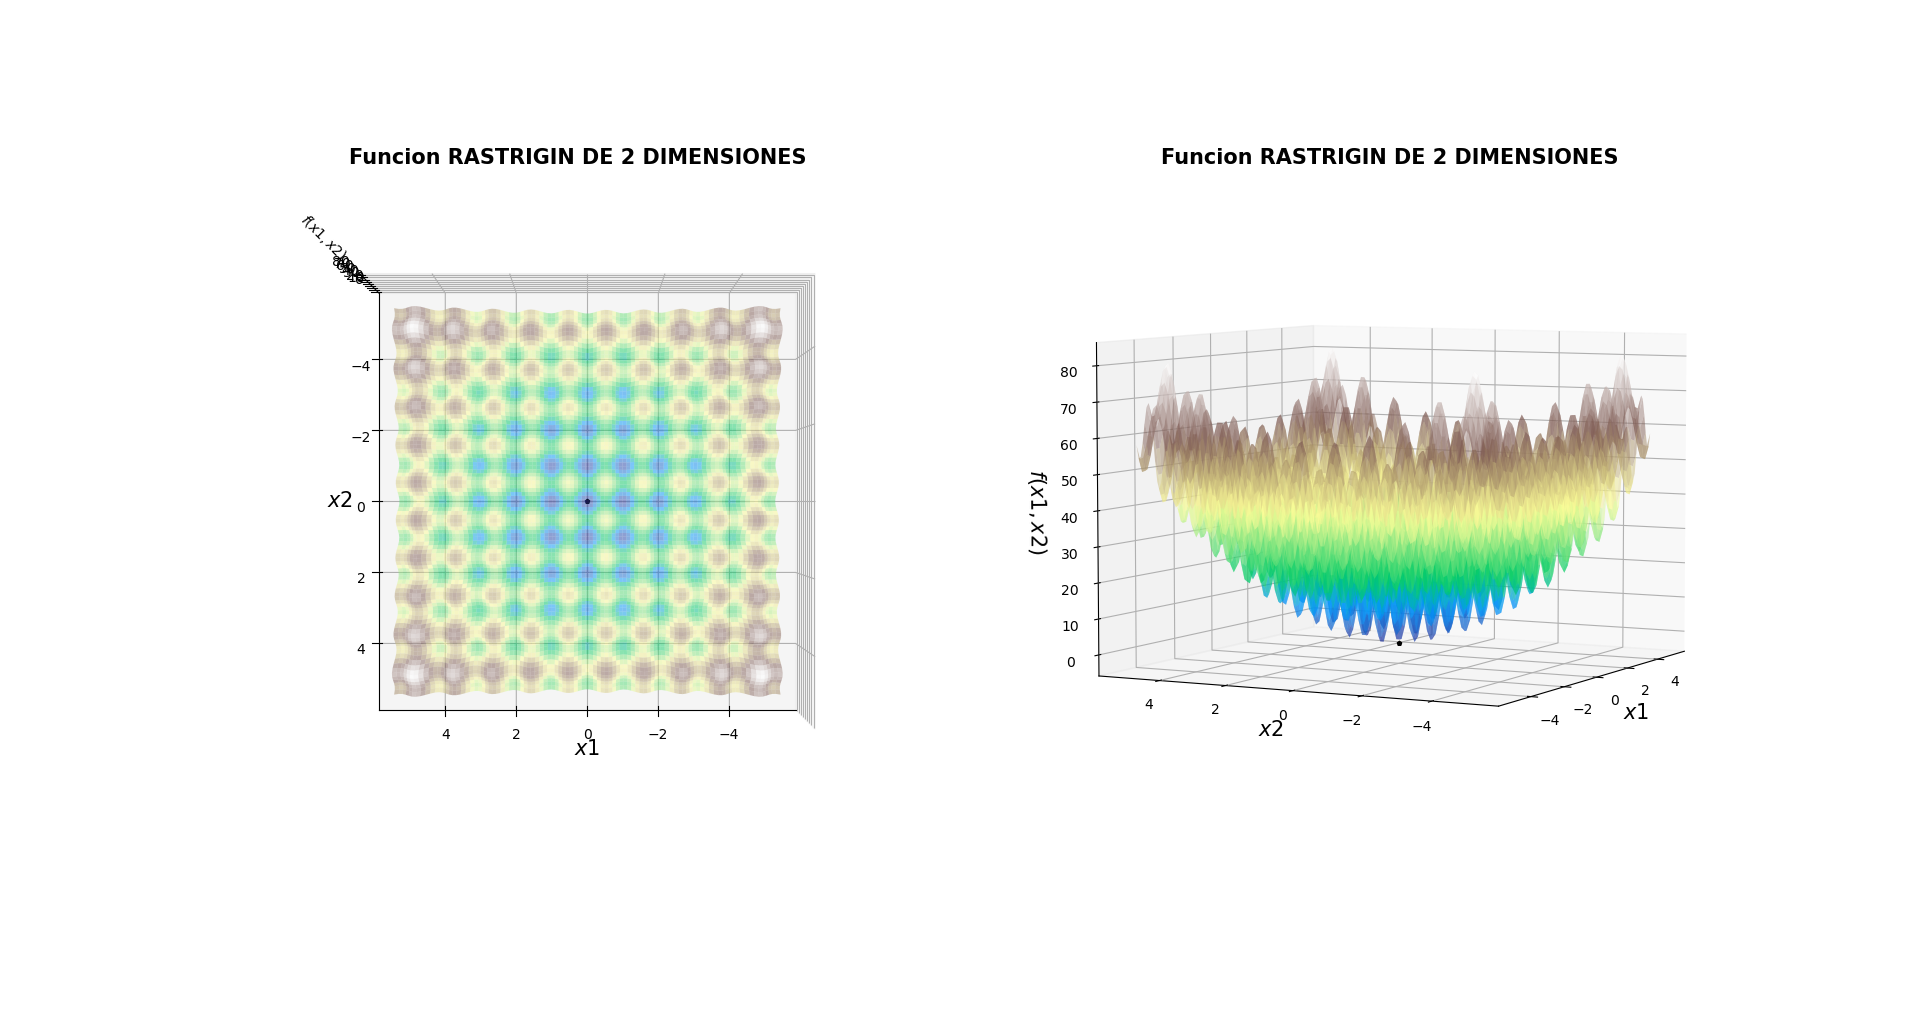
\includegraphics[width=1\textwidth]{C:/Users/anton/Documents/MCIA/UAQ _MCIA/Sem2_Computo_Evolutivo/Prac05_Multi-IslandAGs/Images/Figure_1.png}
    \caption{Representacion bidimensional de funcion Rastrigin, se muestra el minimo global localizado con una estrella negra.}
\end{figure}

\textbf{\large Algoritmos genéticos} 
\\\\
Los algoritmos genéticos parten de la premisa de emplear la evolución natural
como un procedimiento de optimización que se caracteriza por tener operaciones básicas que son:

\begin{itemize}
\item Selección de cromosomas
\item Cruzamiento de cromosomas
\item Mutación de cromosomas
\end{itemize}

Por lo tanto, el algoritmo es una búsqueda empleando dichas operaciones; por ejemplo, se puede plantear una familia de individuos los cuales se seleccionan y después se considera a los mas óptimos para realizar un cruzamiento entre ellos, y la forma de evitar caer en mínimos locales es el empleo de la mutación. Por ello la mutación puede considerarse una operación de fuga de mínimos locales. Esta búsqueda se define como una búsqueda de un espectro amplio.
\\\\
\textbf{\large Métodos de Selección de cromosomas}
\\\\
\begin{itemize}
\item \textbf{Selección por torneo:} se eligen subgrupos de individuos de la población, y los miembros de cada subgrupo compiten entre ellos. Sólo se elige a un individuo de cada subgrupo para la reproducción.

\item \textbf{Selección Rank:} a cada individuo de la población se le asigna un rango numérico basado en su aptitud, y la selección se basa en este ranking, en lugar de las diferencias absolutas en aptitud.

\item \textbf{Selección Random Monogamico:} Cada individuo de la población es seleccionada de manera aleatoria solo una vez y se marca o elimina para que no sea nuevamente utilizado para la cruza. 

\end{itemize}

Estos son los tipos de seleccion de cromosomas que se eligen para la presente practica.
\\\\
\textit{Vectores de números (reales o enteros):} Codificación habitual cuando las variables de nuestro problema son numéricas (codificación directa, aunque habrá que definir operadores genéticos adecuados).

\begin{itemize}
\item Los operadores de cruce (en n puntos y uniforme) se pueden seguir utilizando.

\item El operador de mutación se modifica en función de la
situación:

\begin{itemize}
\item Valores ordinales: Se hace que sea más probable
cambiar a valores cercanos en la escala.

\item Valores categóricos: Selección aleatoria uniforme.	
\end{itemize}

\item Los operadores de cruce y mutación habituales dan lugar a soluciones inadmisibles, por lo que los operadores de mutación deben cambiar al menos dos
valores y los de cruce han de diseñarse específicamente para problemas de este tipo.

\end{itemize}

La probabilidad de mutación ahora se referirá a cromosomas completos, no a genes individuales
\\\\
\textbf{\large Cruzamiento de cromosomas}
\\\\
Operadores de cruce en 2 puntos: Se seleccionan dos puntos para cortar un cromosoma y después se juntan los fragmentos alternando los cromosomas 1 y 2.

\[( \;1\;|\;2\;3\;4\;5\;|\;6\;7\;8\;9\; )\;\;  ( \;1\;|\;8\;7\;6\;5\;|\;6\;7\;8\;9\; )\]

\[( \;9\;|\;8\;7\;6\;5\;|\;4\;3\;2\;1\; )\;\;  ( \;9\;|\;2\;3\;4\;5\;|\;4\;3\;2\;1\; )\]

Operadores de cruce en N puntos: Se seleccionan N puntos para cortar un cromosoma y después se juntan los fragmentos alternando los cromosomas 1 y 2.

\[( \;1\;|\;2\;3\;|\;4\;5\;|\;6\;7\;8\;9\; )\;\;  ( \;1\;|\;8\;7\;|\;4\;5\;|\;4\;3\;2\;1\; )\]

\[( \;9\;|\;8\;7\;|\;6\;5\;|\;4\;3\;2\;1\; )\;\;  ( \;9\;|\;2\;3|\;\;6\;5\;|\;6\;7\;8\;9\; )\]
\textbf{\large Mutación}
\\\\
\textbf{Operadores de mutación}
\\\\
\begin{itemize}
\item \textbf{Inserción: }Elegir dos alelos aleatoriamente y colocar el segundo justo después del primero.
\[( \;1\;|\;2\;|\;\;3\;4\;|\;5\;|\;6\;7\;8\;9\; ) ---> ( \;1\;|\;2\;5\;|\;3\;4\;6\;7\;8\;9\; )\]
\item \textbf{Intercambio: }Seleccionar dos alelos aleatoriamente e intercambiarlos.
\[( \;1\;|\;2\;|\;3\;4\;|\;5\;|\;6\;7\;8\;9\; ) ---> ( \;1\;|\;5\;|\;3\;4\;|\;2\;|\;6\;7\;8\;9\; )\]
\item \textbf{Inversión: }Seleccionar dos alelos aleatoriamente e invertir la cadena entre ellos.

\[( \;1\;|\;2\;3\;4\;5\;|\;6\;7\;8\;9\; ) ---> ( \;1\;|\;5\;4\;3\;2\;|\;6\;7\;8\;9\; )\]

\item \textbf{Revuelto[Scramble]}Seleccionar un subconjunto de genes y reordenar aleatoriamente los alelos (el subconjunto no tiene por qué ser contiguo).

\[( \;1\;|\;2\;3\;4\;5\;|\;6\;7\;8\;9\; ) ---> ( \;1\;|\;3\;5\;4\;2\;|\;6\;7\;8\;9\; )\]

\end{itemize}

Se observa como cada operador de mutación afecta de forma diferente al orden relativo y a las relaciones de adyacencia.

\section{Materiales}
Computadora personal portátil MSI, procesador Intel(R)Core(TM) i7-750H CPU @ 2.60GHz, 16GB de memoria RAM, Sistema operativo Windows 10 de 64 bits, Software: Jupyter Notebook y entorno Anaconda, lenguaje Python.

\section{Metodología}
El algoritmo desarrollado es como sigue:
\\\\
\hrulefill \textit{Definicion de parametros de islas} \\
\hspace*{1cm}\textit{Num generaciones}\\
\hspace*{1cm}\textit{Cantidad de isleños}\\
\hspace*{1cm}\textit{Tipo Seleccion, cruza y mutacion para cada isla}\\
\hspace*{1cm}\textit{Definicion de ejecucion de migraciones}\\
\textit{Creacion de isleños}\\
\hspace*{1cm}\textit{Evaluación cromosomas}\\
\hspace*{1cm}\textit{Ordenación por criterio elitista}\\
\textit{for epsilon $<$90\% or iteración $>$ a Generaciones}\\
\hspace*{1cm}\textit{Llamada a isla1}	\\
\hspace*{1cm}\textit{Llamada a isla2}	\\
\hspace*{1cm}\textit{Llamada a isla3}	\\
\hspace*{1cm}\textit{if generaciones \% seasons1==0}\\
\hspace*{2cm}\textit{Eleccion de isla mejor y peor}	\\
\hspace*{2cm}\textit{Intercambio de isleños entre ellos}\\
\hspace*{1cm}\textit{if generaciones \% seasons2==0}\\
\hspace*{2cm}\textit{Intercambio circular de isleño entre islas}	\\
\hspace*{1cm}\textit{if generaciones \% seasons3==0}\\
\hspace*{2cm}\textit{Eleccion de isleño para visitar isla}	\\
\hspace*{2cm}\textit{Cruza con individuo de isla visitada}	\\
\hspace*{2cm}\textit{Retorno de isleño}	\\
\hspace*{1cm}\textit{Verificacion de isleños por isla}\\
\hspace*{1cm}\textit{Ordenamiento por aptitud}\\
\hspace*{1cm}\textit{Se repite for}\\
\textit{Graficación de resultados}\\
\textit{Fin}\\
\\\\
La ejecucion del algoritmo se propone de manera secuencial, primero se ejecuta una isla se guardan sus resultados y se continua con la siguiente. Cuando se termina de ejecutar las 3 islas se procede a realizar las migraciones en caso de que sea necesario dado las generaciones que lleva el contador $for$, al final se reordena los datos de cada isla para manejar los cambios que se realizaron debido a las migraciones.
\\\\
La definicion de generaciones se definen al mismo tiempo que el tipo de cruza, seleccion y mutacion. Posteriormente se crean las poblaciones para cada isla, como se muestra en la seccion de codigo de la figura 2.

\begin{figure}[H]
	\centering
    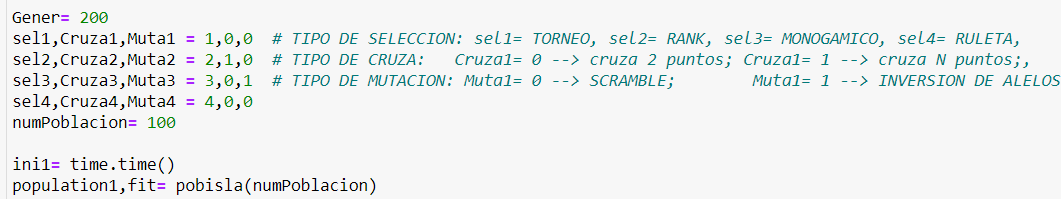
\includegraphics[width=1\textwidth]{C:/Users/anton/Documents/MCIA/UAQ _MCIA/Sem2_Computo_Evolutivo/Prac05_Multi-IslandAGs/Images/Figure_2.png}
    \caption{Seccion de codigo de definicion de parametros.}
\end{figure}
 
La implementacion de multi-islas se realiza con el fin de compartir informacion entre las islas, esto para poder resolver una tarea "dividiendo el trabajo" con el fin de alcanzar un optimo de forma mas eficiente.
\\\\
Para ello se proponen tres tipos de migracion:

\begin{itemize}
\item Migracion Mejor/Peor: Se migran varios isleños de la isla con mejor promedio a la de peor promedio, para poder mejorar su promedio

\item Migracion Circular: Se migran varios pobladores entre las islas de manera circular, esto para que compartan informacion entre todas las islas. La isla 1 migra n isleños a la isla 2 y a su vez recibe de otra isla para complementar los que migraron. Se reacondiciona en caso de mas islas.

\item Visitante Marinero: Un isleño de cierta isla "visita" otra isla en la que se cruza con un isleño de la isla visitada eliminando n isleños para balancear la cantidad de isleños. Despues el isleño visitante regresa a su isla.

\end{itemize}
Las migraciones ocurren cada 6 generaciones para migrar de mejor isla a peor, 3 para migrar de manera circular y 7 generaciones para visita de isleño. Tambien se define la tolerancia DELTA de paro. Como se muestra en la seccion de codigo de la figura 3.

\begin{figure}[H]
	\centering
    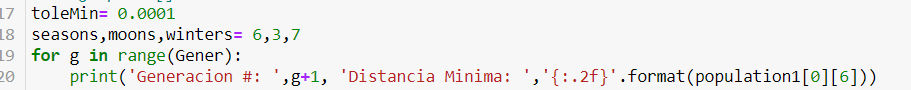
\includegraphics[width=1\textwidth]{C:/Users/anton/Documents/MCIA/UAQ _MCIA/Sem2_Computo_Evolutivo/Prac05_Multi-IslandAGs/Images/Figure_3.png}
    \caption{Seccion de codigo de definicion de tiempo de migraciones.}
\end{figure}
\newpage
\section{Resultados y discusión}
Se realizaron 4 pruebas variando los parametros como numero de isleños, tipo de cruza y tipo de mutacion para cada tipo de Seleccion, se establecio un 5\% de individuos para mutacion de cada poblacion, una tolerancia Delta de 0.0001 para asegurar que se llega al minimo global con 12 cifras y las generaciones se mantuvieron en 200.
\\\\
Primero se realizaron las pruebas a las isla sin interaccion entre ellas, esto es, que no hubo migracion entre ellas, para poder hacer comparaciones cuando posteriormente se llevaron a cabo las mismas prubas pero con migracion entre islas. Las graficas de la figura 4 muestran los resultados obtenidos.

\begin{figure}[H]
      \begin{center}
        \subfigure[Seleccion Torneo]{
            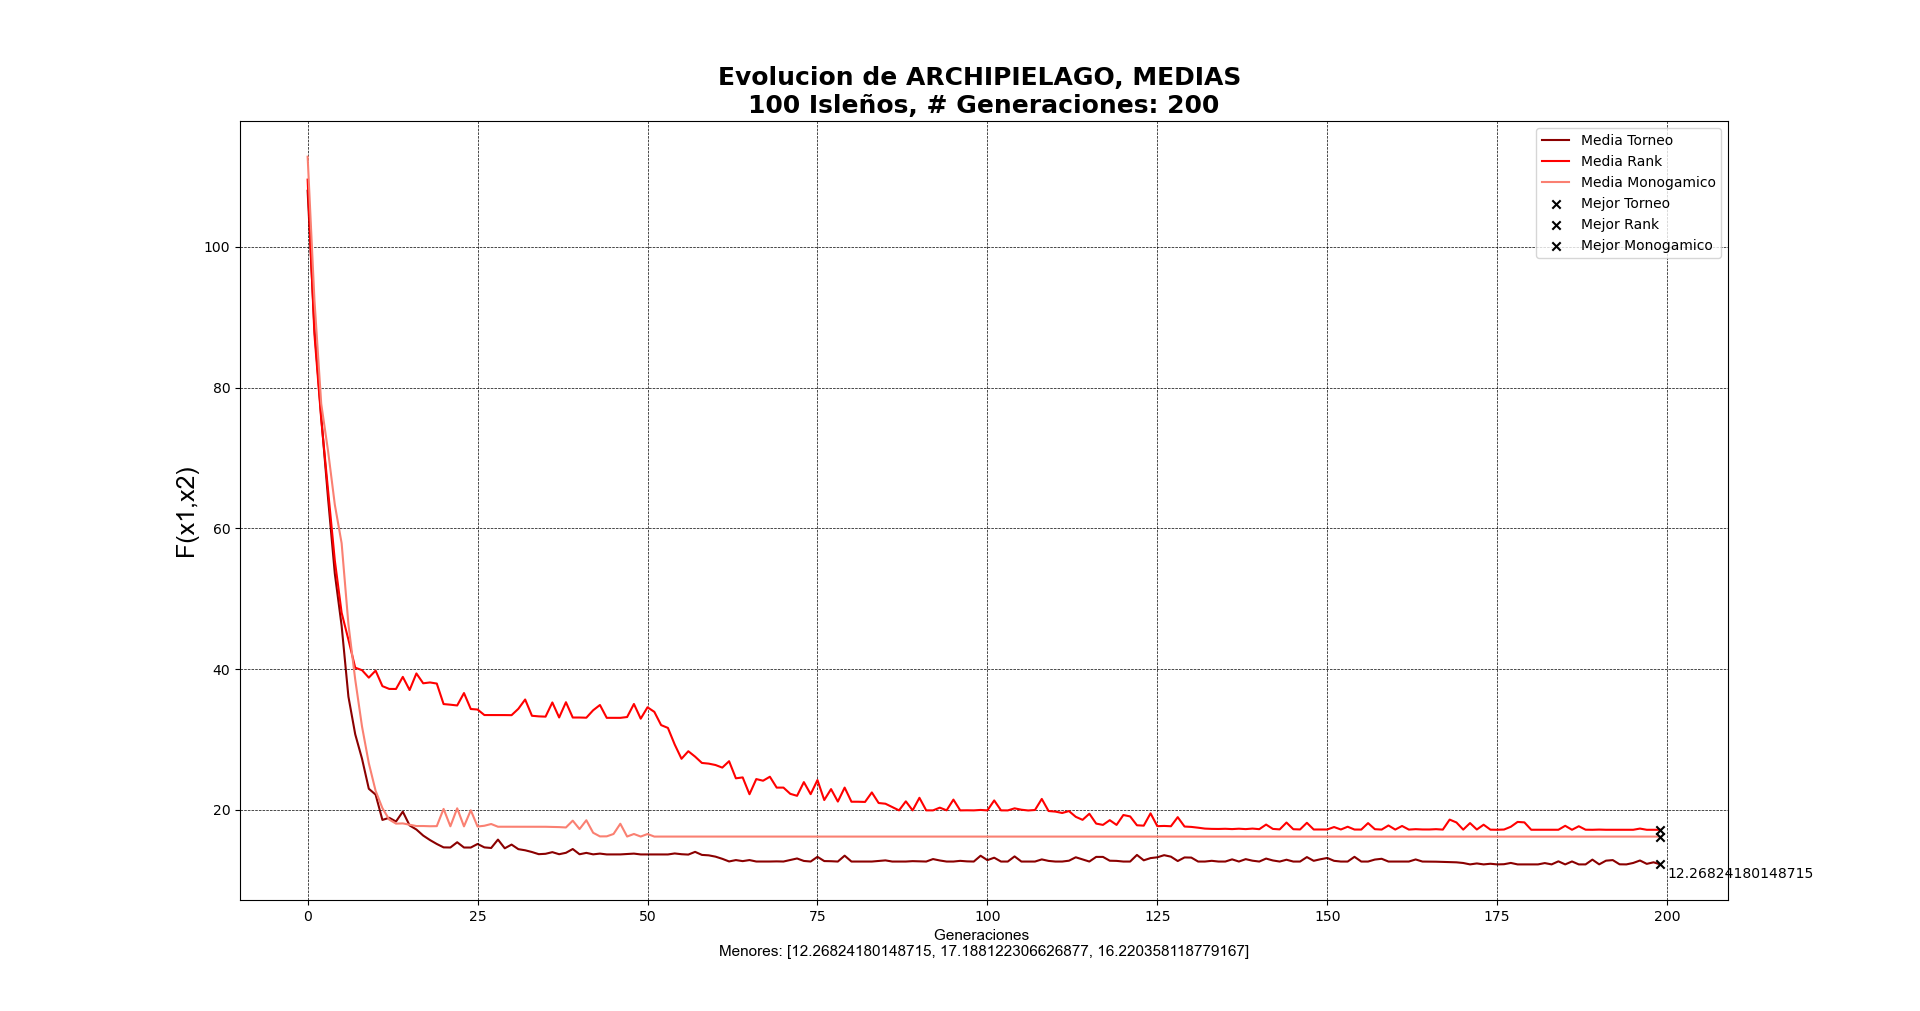
\includegraphics[width=0.85\textwidth]{C:/Users/anton/Documents/MCIA/UAQ _MCIA/Sem2_Computo_Evolutivo/Prac05_Multi-IslandAGs/Images/Figure_4.png}
            \label{Señal 1}}
        \subfigure[Evolucion de las medias de las islas]{
            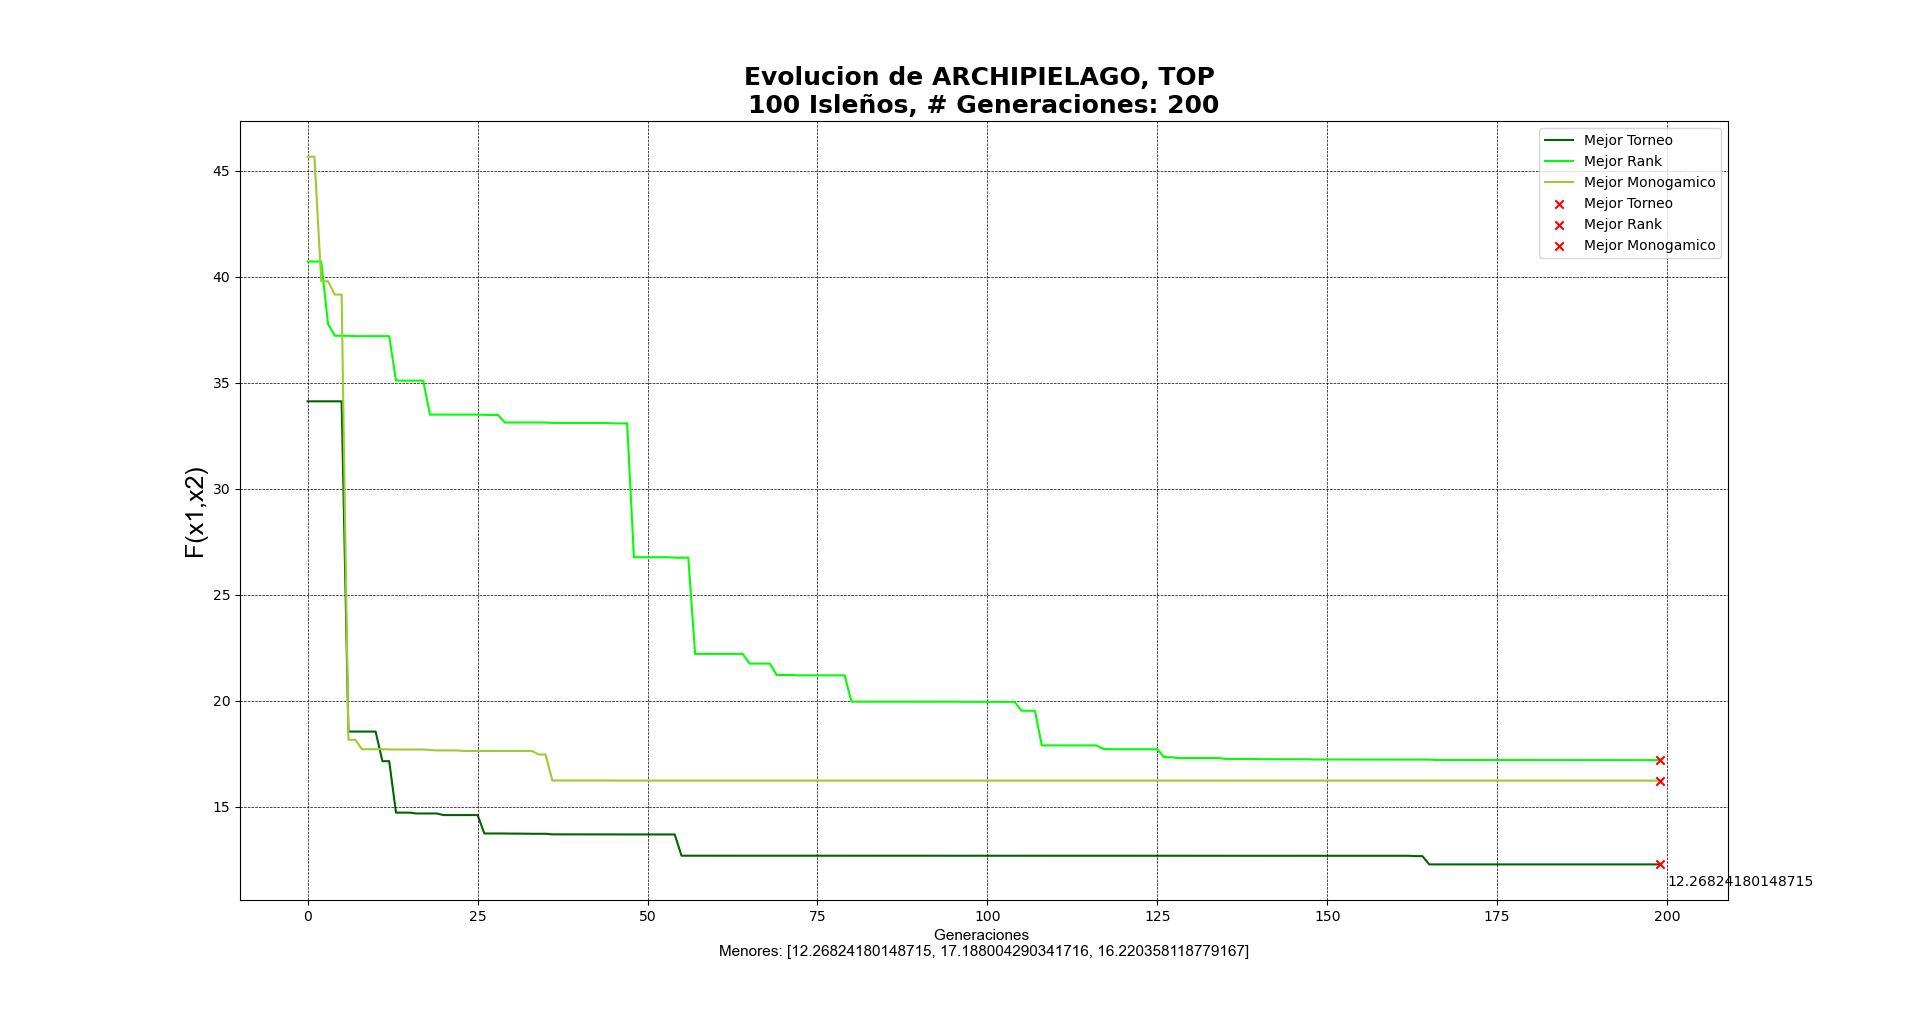
\includegraphics[width=0.85\textwidth]{C:/Users/anton/Documents/MCIA/UAQ _MCIA/Sem2_Computo_Evolutivo/Prac05_Multi-IslandAGs/Images/Figure_5.png}
            \label{Señal 2}}
        \caption{Evolucion del mejor de las islas}
        \label{Patron de señales para reconocimiento de señal Gaussiana}
      \end{center}
    \end{figure}

Parametros establecidos para prueba 1 son:
\\
\textbf{Isla 1:} Numero de Isleños: 100\\
Seleccion: Torneo\\ 
Tipo de cruza: cruza 2 puntos\\
Tipo de mutacion: Scramble\\
\textbf{Isla 2:} Numero de Isleños: 100\\
Seleccion: Torneo\\ 
Tipo de cruza: cruza N puntos\\
Tipo de mutacion: Scramble\\
\textbf{Isla 3:} Numero de Isleños: 100\\
Seleccion: Torneo\\ 
Tipo de cruza: cruza 2 puntos\\
Tipo de mutacion: Inversion de alelos

\begin{figure}[H]
      \begin{center}
        \subfigure[Seleccion Torneo]{
            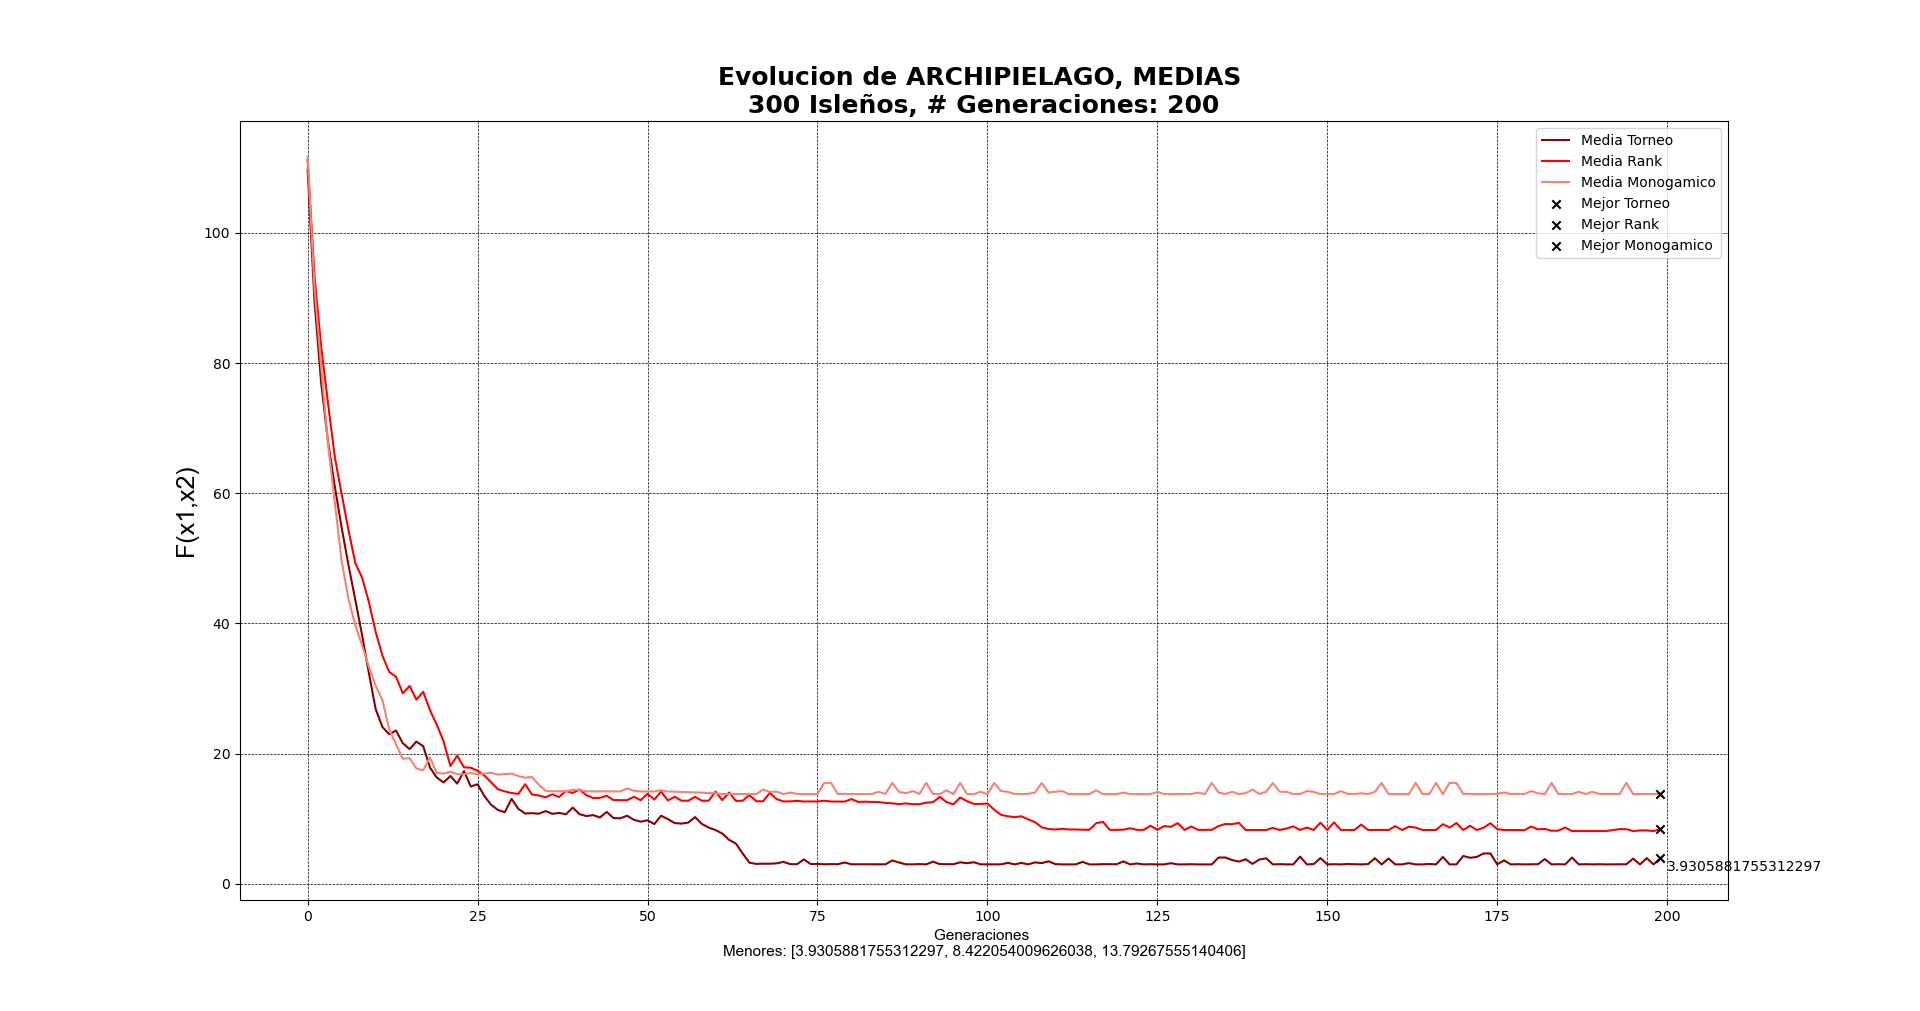
\includegraphics[width=0.85\textwidth]{C:/Users/anton/Documents/MCIA/UAQ _MCIA/Sem2_Computo_Evolutivo/Prac05_Multi-IslandAGs/Images/Figure_7.png}
            \label{Señal 1}}
        \subfigure[Evolucion de las medias de las islas]{
            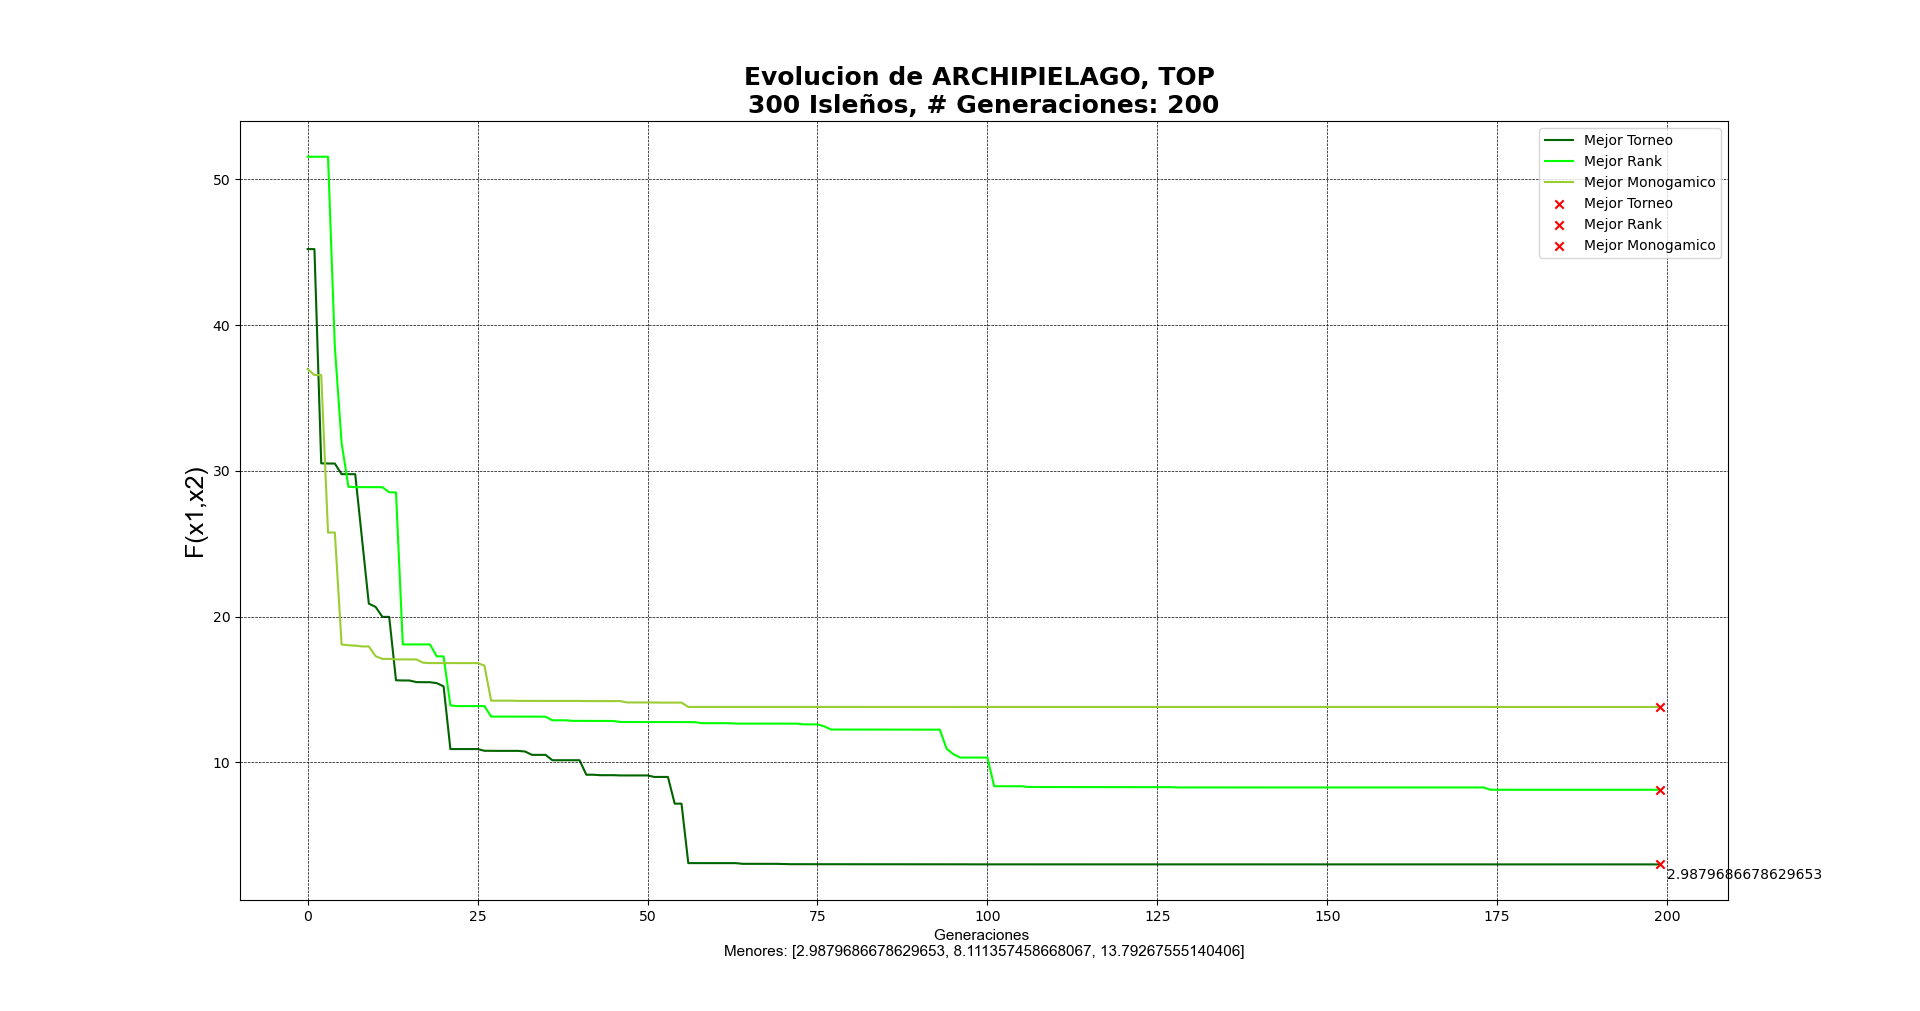
\includegraphics[width=0.85\textwidth]{C:/Users/anton/Documents/MCIA/UAQ _MCIA/Sem2_Computo_Evolutivo/Prac05_Multi-IslandAGs/Images/Figure_8.png}
            \label{Señal 2}}
        \caption{Evolucion del mejor de las islas}
        \label{Patron de señales para reconocimiento de señal Gaussiana}
      \end{center}
    \end{figure}

Parametros establecidos para prueba 2 son:
\\
\textbf{Isla 1:} Numero de Isleños: 300\\
Seleccion: Torneo\\ 
Tipo de cruza: cruza 2 puntos\\
Tipo de mutacion: Scramble\\
\textbf{Isla 2:} Numero de Isleños: 300\\
Seleccion: Torneo\\ 
Tipo de cruza: cruza N puntos\\
Tipo de mutacion: Scramble\\
\textbf{Isla 3:} Numero de Isleños: 300\\
Seleccion: Torneo\\ 
Tipo de cruza: cruza 2 puntos\\
Tipo de mutacion: Inversion de alelos

\begin{figure}[H]
      \begin{center}
        \subfigure[Seleccion Torneo]{
            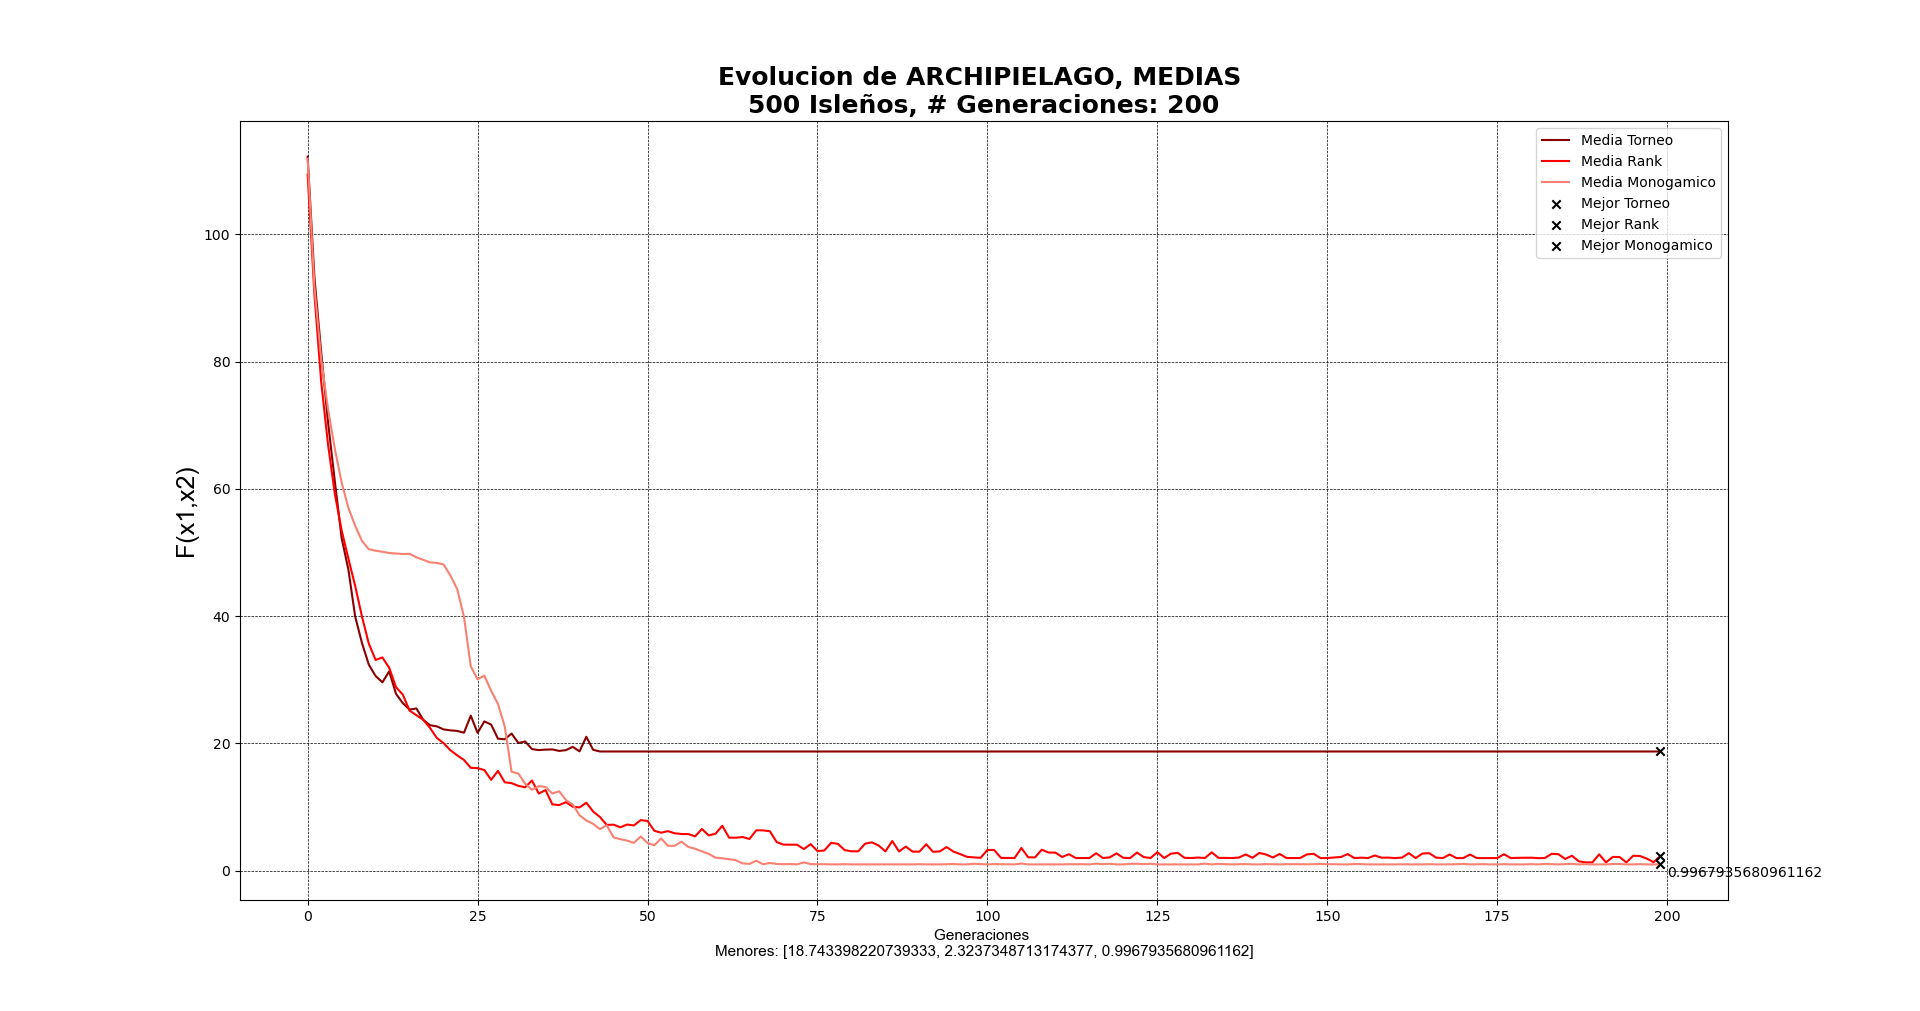
\includegraphics[width=0.85\textwidth]{C:/Users/anton/Documents/MCIA/UAQ _MCIA/Sem2_Computo_Evolutivo/Prac05_Multi-IslandAGs/Images/Figure_11.png}
            \label{Señal 1}}
        \subfigure[Evolucion de las medias de las islas]{
            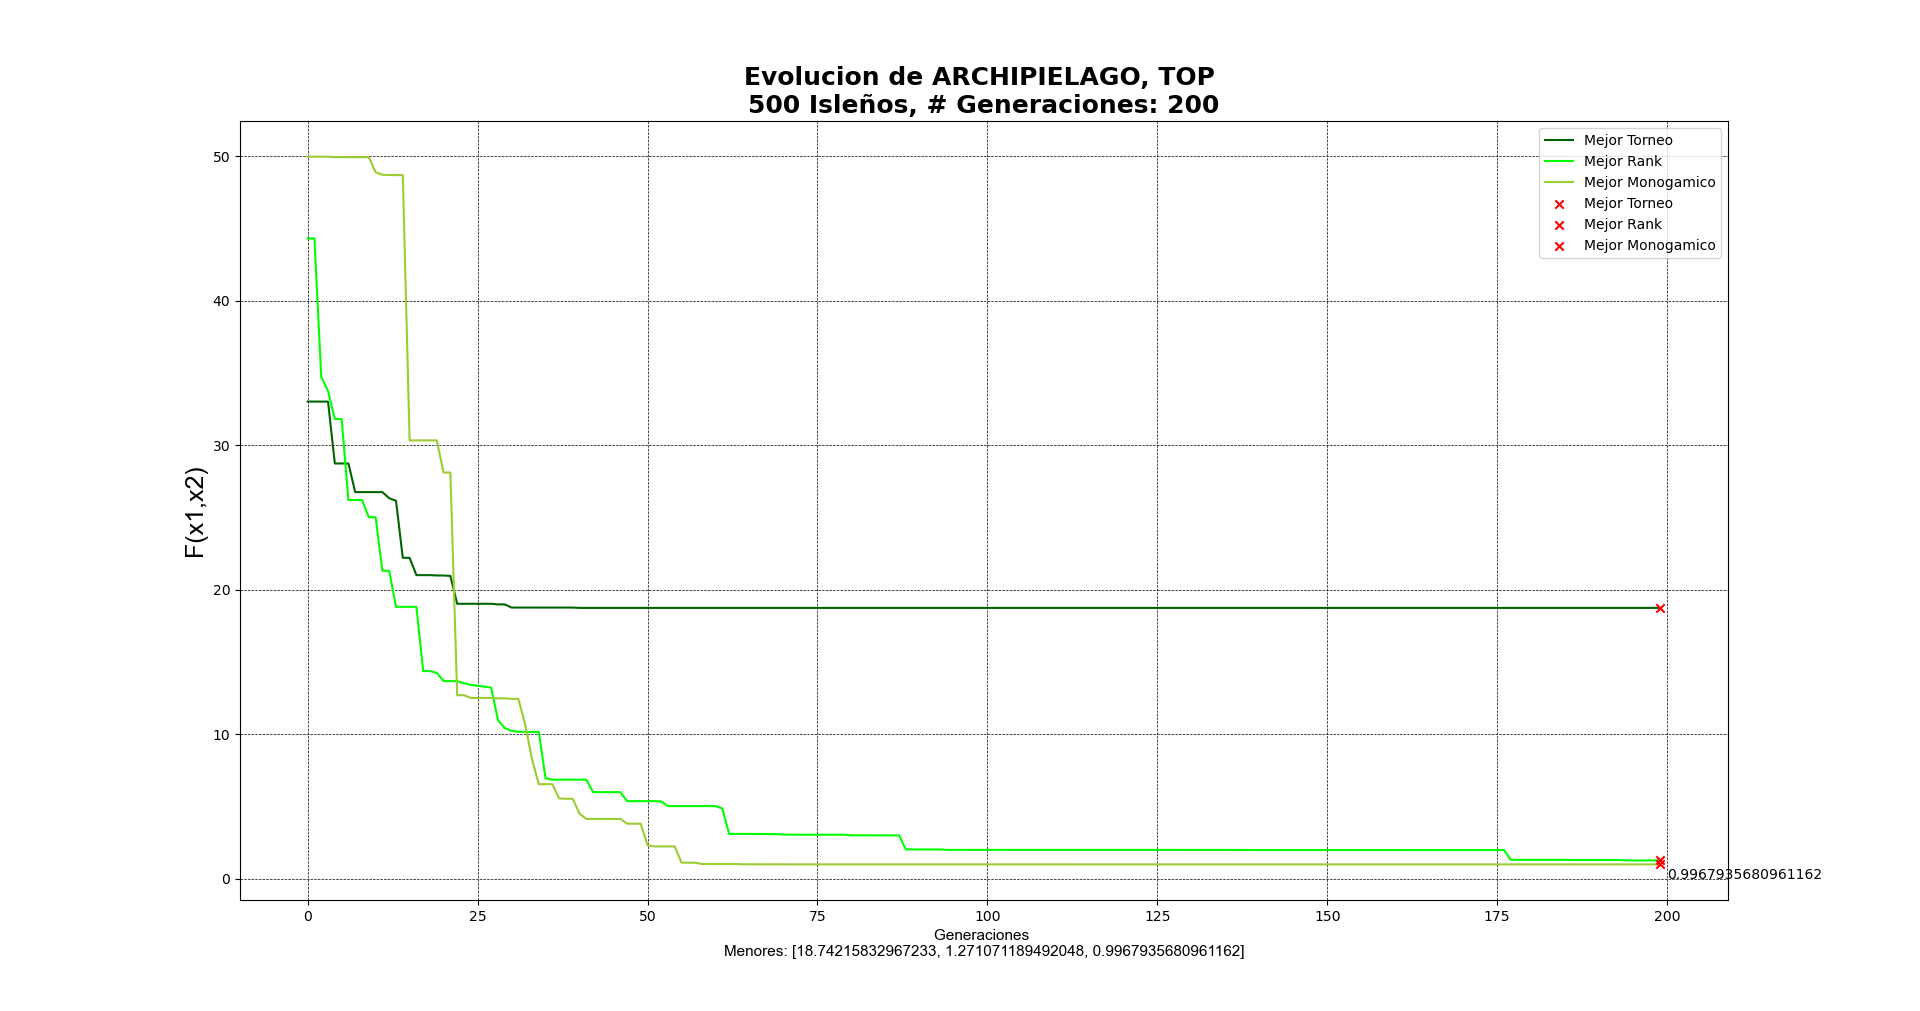
\includegraphics[width=0.85\textwidth]{C:/Users/anton/Documents/MCIA/UAQ _MCIA/Sem2_Computo_Evolutivo/Prac05_Multi-IslandAGs/Images/Figure_12.png}
            \label{Señal 2}}
        \caption{Evolucion del mejor de las islas}
        \label{Patron de señales para reconocimiento de señal Gaussiana}
      \end{center}
    \end{figure}

Parametros establecidos para prueba 3 son:
\\
\textbf{Isla 1:} Numero de Isleños: 500\\
Seleccion: Torneo\\ 
Tipo de cruza: cruza 2 puntos\\
Tipo de mutacion: Inversion de Alelos\\
\textbf{Isla 2:} Numero de Isleños: 500\\
Seleccion: Torneo\\ 
Tipo de cruza: cruza N puntos\\
Tipo de mutacion: Scramble\\
\textbf{Isla 3:} Numero de Isleños: 500\\
Seleccion: Torneo\\ 
Tipo de cruza: cruza 2 puntos\\
Tipo de mutacion: Scramble

\begin{figure}[H]
      \begin{center}
        \subfigure[Seleccion Torneo]{
            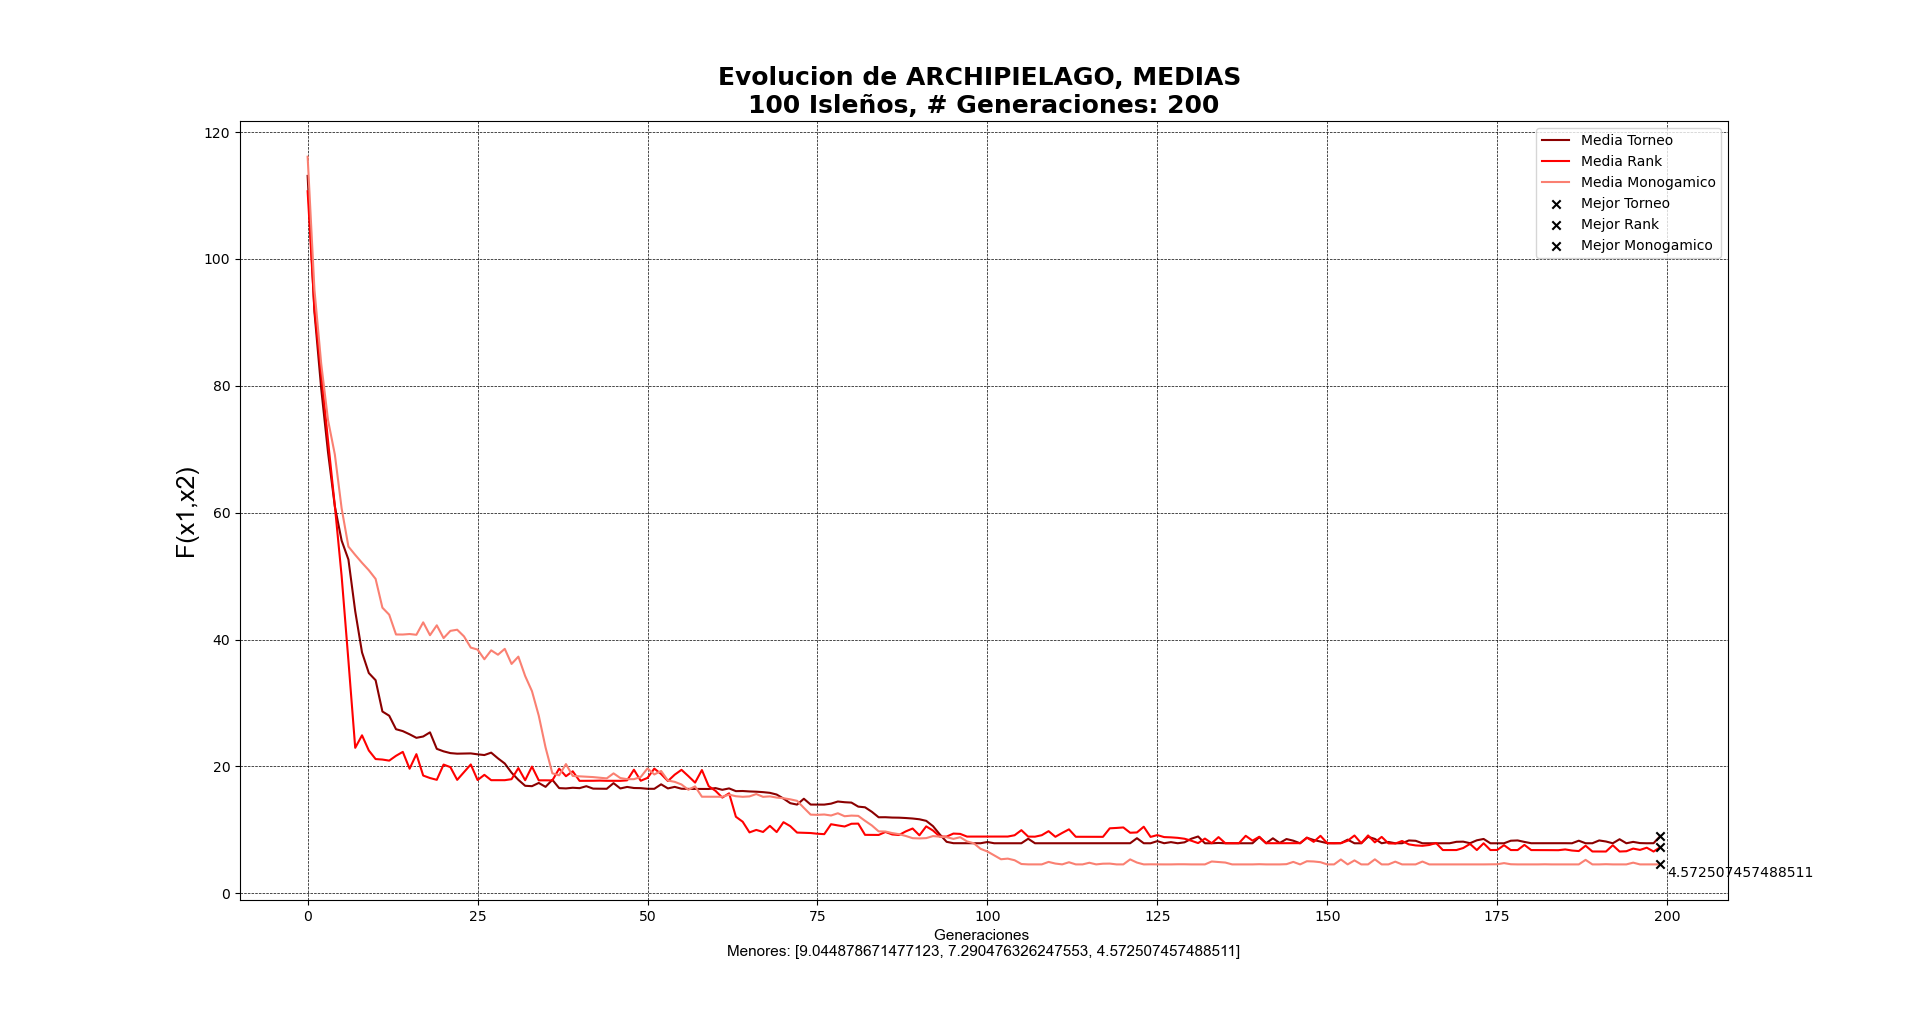
\includegraphics[width=0.85\textwidth]{C:/Users/anton/Documents/MCIA/UAQ _MCIA/Sem2_Computo_Evolutivo/Prac05_Multi-IslandAGs/Images/Figure_15.png}
            \label{Señal 1}}
        \subfigure[Evolucion de las medias de las islas]{
            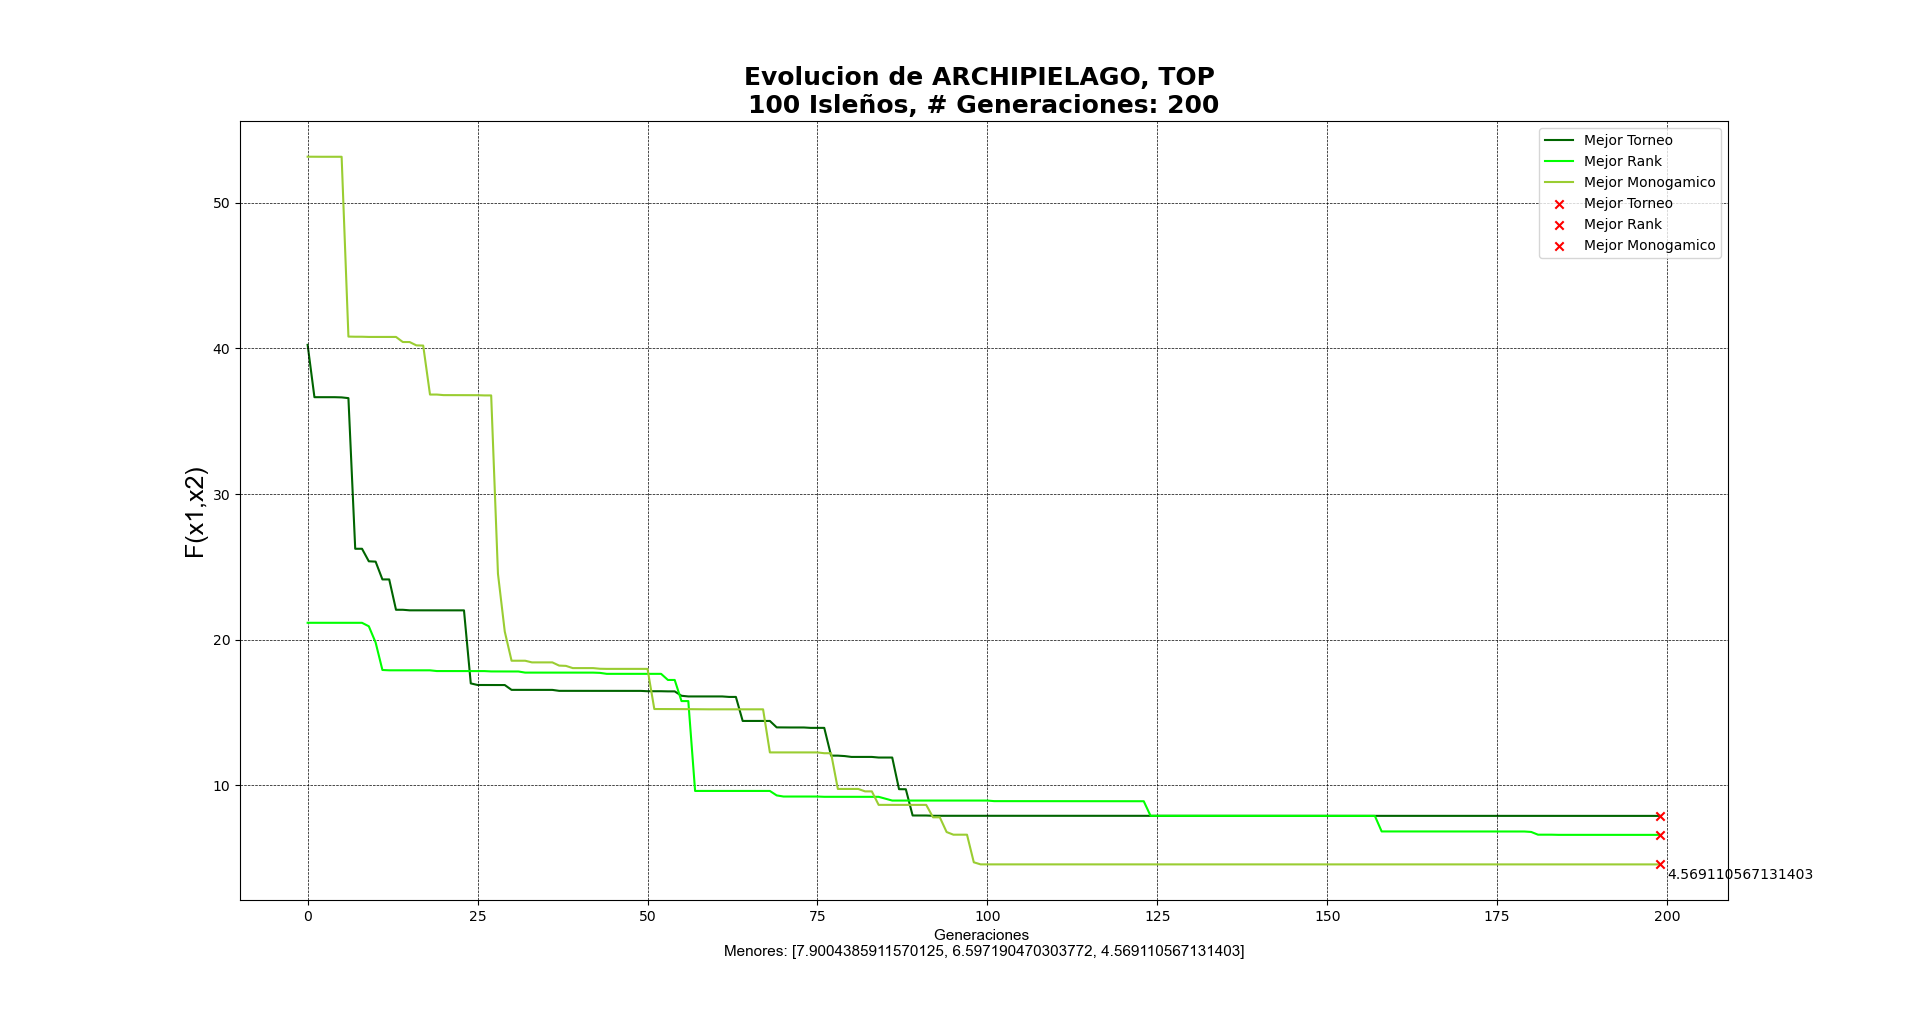
\includegraphics[width=0.85\textwidth]{C:/Users/anton/Documents/MCIA/UAQ _MCIA/Sem2_Computo_Evolutivo/Prac05_Multi-IslandAGs/Images/Figure_16.png}
            \label{Señal 2}}
        \caption{Evolucion del mejor de las islas}
        \label{Patron de señales para reconocimiento de señal Gaussiana}
      \end{center}
    \end{figure}

Parametros establecidos para prueba 4 son:
\\
\textbf{Isla 1:} Numero de Isleños: 100\\
Seleccion: Torneo\\ 
Tipo de cruza: cruza 2 puntos\\
Tipo de mutacion: Scramble\\
\textbf{Isla 2:} Numero de Isleños: 100\\
Seleccion: Torneo\\ 
Tipo de cruza: cruza 2 puntos\\
Tipo de mutacion: Scramble\\
\textbf{Isla 3:} Numero de Isleños: 100\\
Seleccion: Torneo\\ 
Tipo de cruza: cruza 2 puntos\\
Tipo de mutacion: Scramble
\\\\
\textbf{\large Pruebas realizadas con migracion entre islas}
\\\\
Parametros establecidos para prueba 1 son:
\\
\textbf{Isla 1:} Numero de Isleños: 100\\
Seleccion: Torneo\\ 
Tipo de cruza: cruza 2 puntos\\
Tipo de mutacion: Scramble\\
\textbf{Isla 2:} Numero de Isleños: 100\\
Seleccion: Torneo\\ 
Tipo de cruza: cruza N puntos\\
Tipo de mutacion: Scramble\\
\textbf{Isla 3:} Numero de Isleños: 100\\
Seleccion: Torneo\\ 
Tipo de cruza: cruza 2 puntos\\
Tipo de mutacion: Inversion de alelos

\begin{figure}[H]
      \begin{center}
        \subfigure[Seleccion Torneo]{
            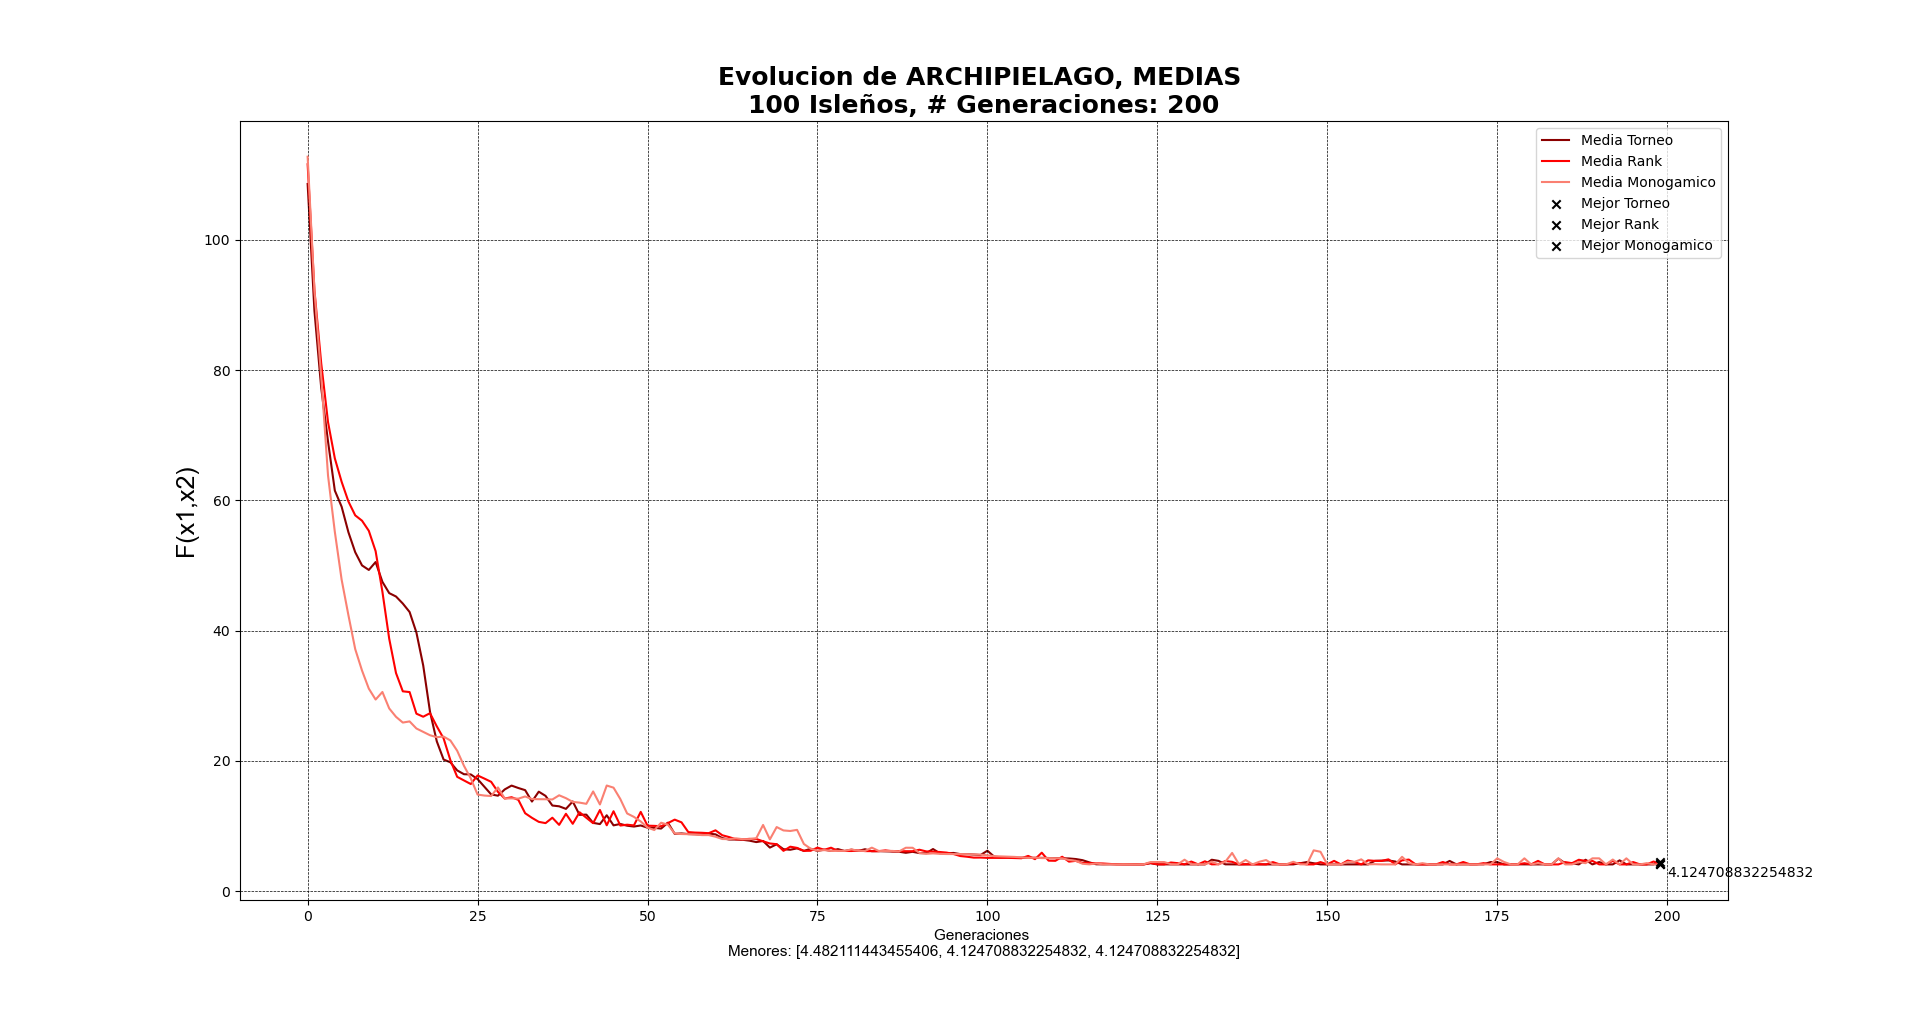
\includegraphics[width=0.85\textwidth]{C:/Users/anton/Documents/MCIA/UAQ _MCIA/Sem2_Computo_Evolutivo/Prac05_Multi-IslandAGs/Images/Figure_19.png}
            \label{Señal 1}}
        \subfigure[Evolucion de las medias de las islas]{
            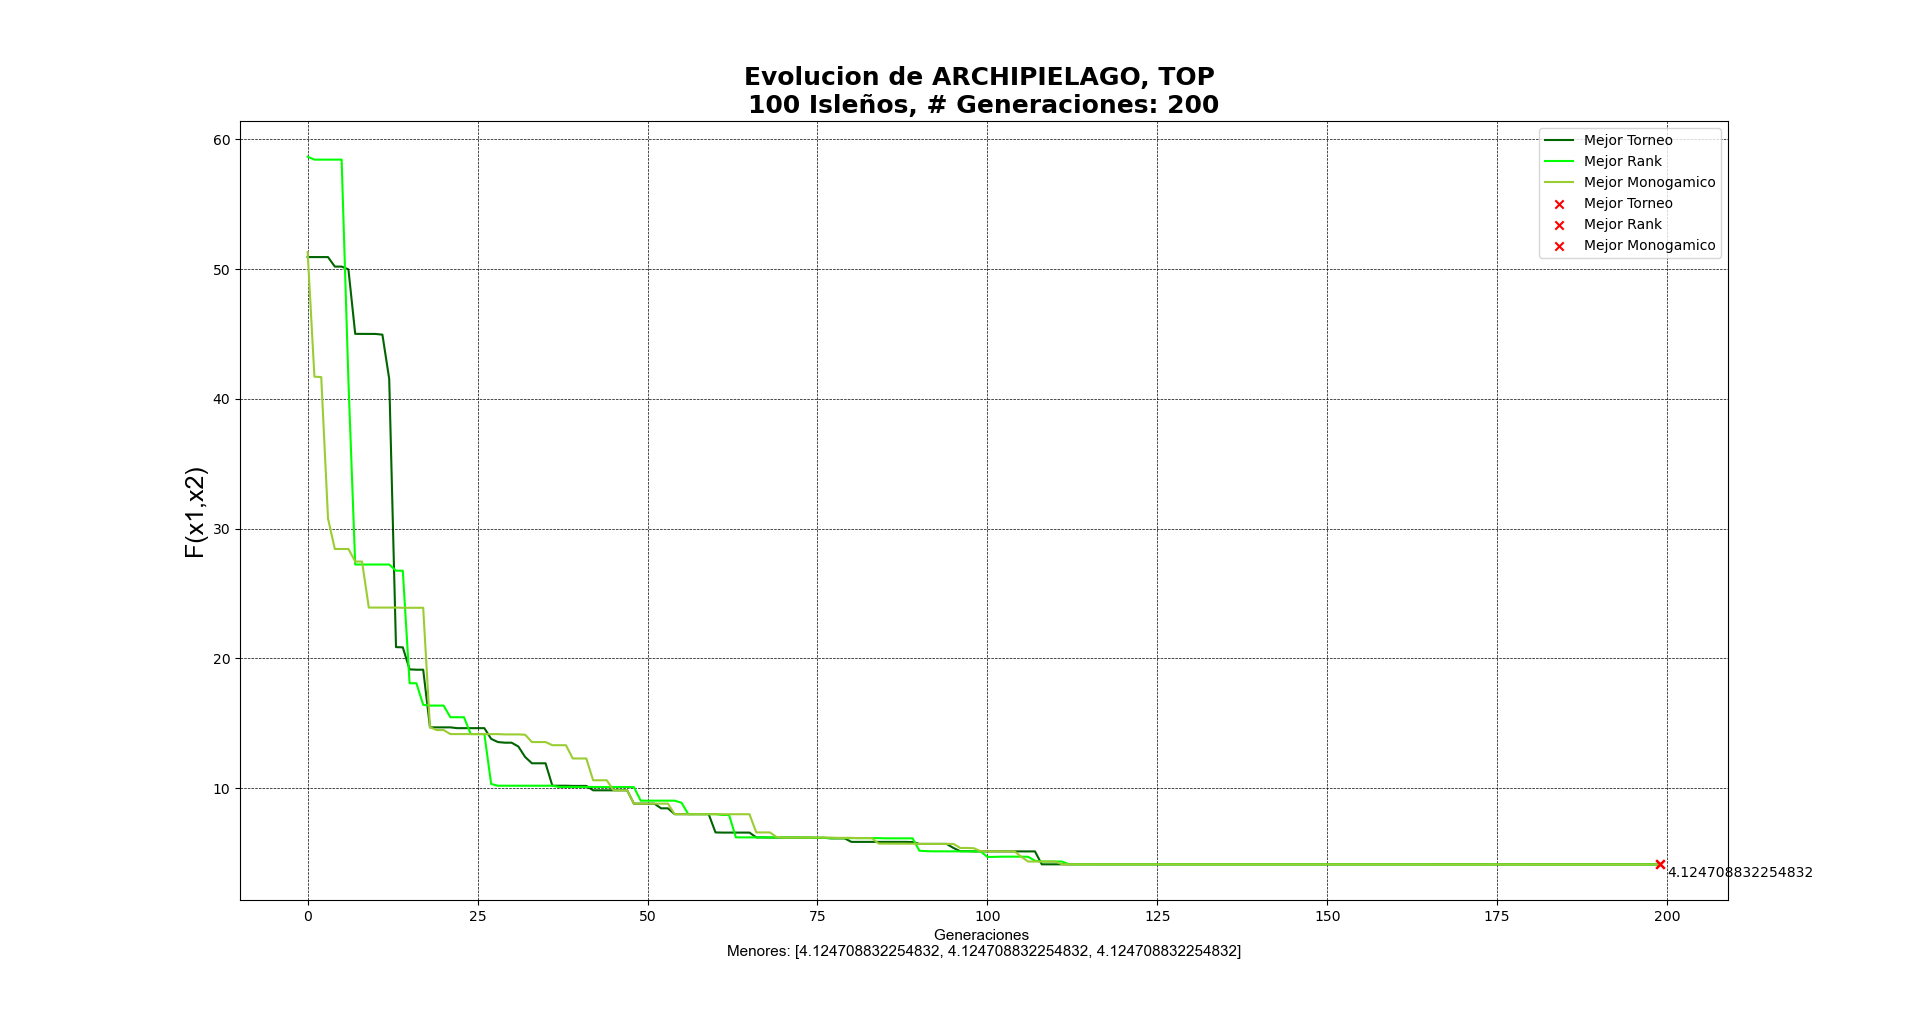
\includegraphics[width=0.85\textwidth]{C:/Users/anton/Documents/MCIA/UAQ _MCIA/Sem2_Computo_Evolutivo/Prac05_Multi-IslandAGs/Images/Figure_20.png}
            \label{Señal 2}}
        \caption{Evolucion del mejor de las islas}
        \label{Patron de señales para reconocimiento de señal Gaussiana}
      \end{center}
    \end{figure}

Parametros establecidos para prueba 2 son:
\\
\textbf{Isla 1:} Numero de Isleños: 300\\
Seleccion: Torneo\\ 
Tipo de cruza: cruza 2 puntos\\
Tipo de mutacion: Scramble\\
\textbf{Isla 2:} Numero de Isleños: 300\\
Seleccion: Torneo\\ 
Tipo de cruza: cruza N puntos\\
Tipo de mutacion: Scramble\\
\textbf{Isla 3:} Numero de Isleños: 300\\
Seleccion: Torneo\\ 
Tipo de cruza: cruza 2 puntos\\
Tipo de mutacion: Inversion de alelos

\begin{figure}[H]
      \begin{center}
        \subfigure[Seleccion Torneo]{
            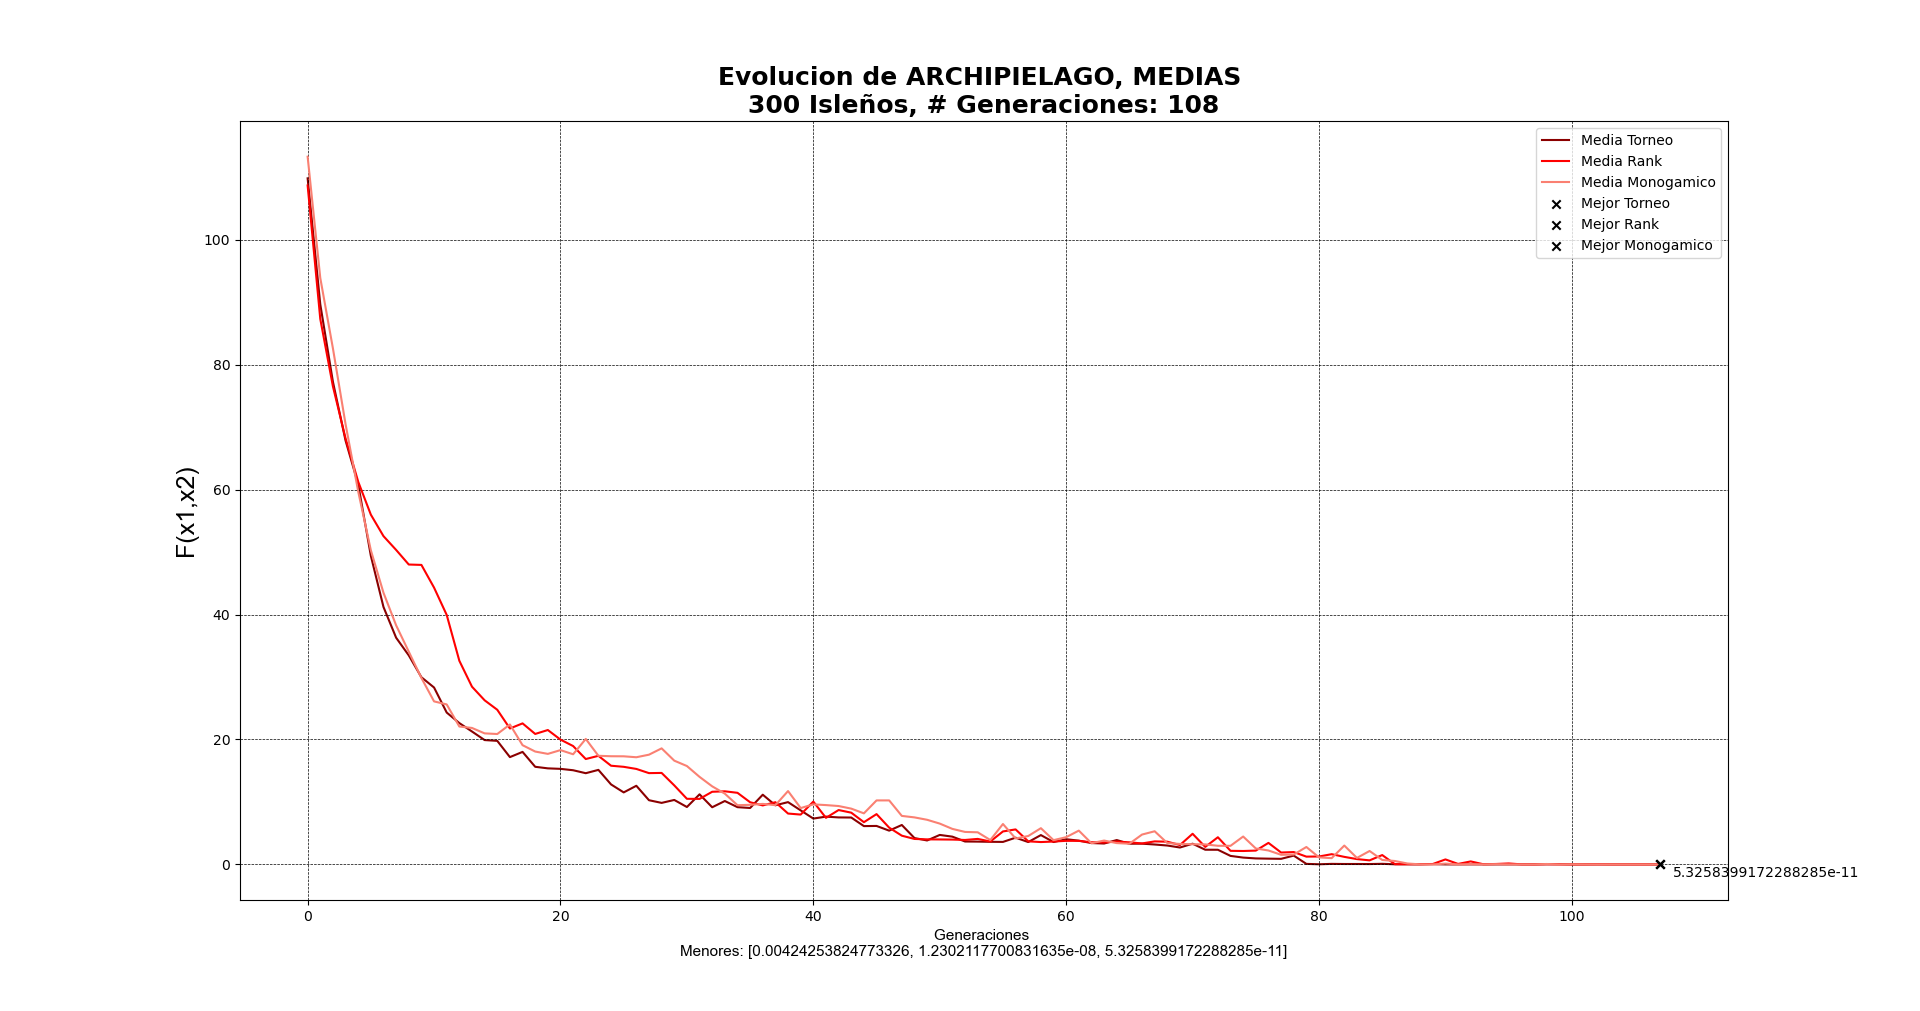
\includegraphics[width=0.85\textwidth]{C:/Users/anton/Documents/MCIA/UAQ _MCIA/Sem2_Computo_Evolutivo/Prac05_Multi-IslandAGs/Images/Figure_23.png}
            \label{Señal 1}}
        \subfigure[Evolucion de las medias de las islas]{
            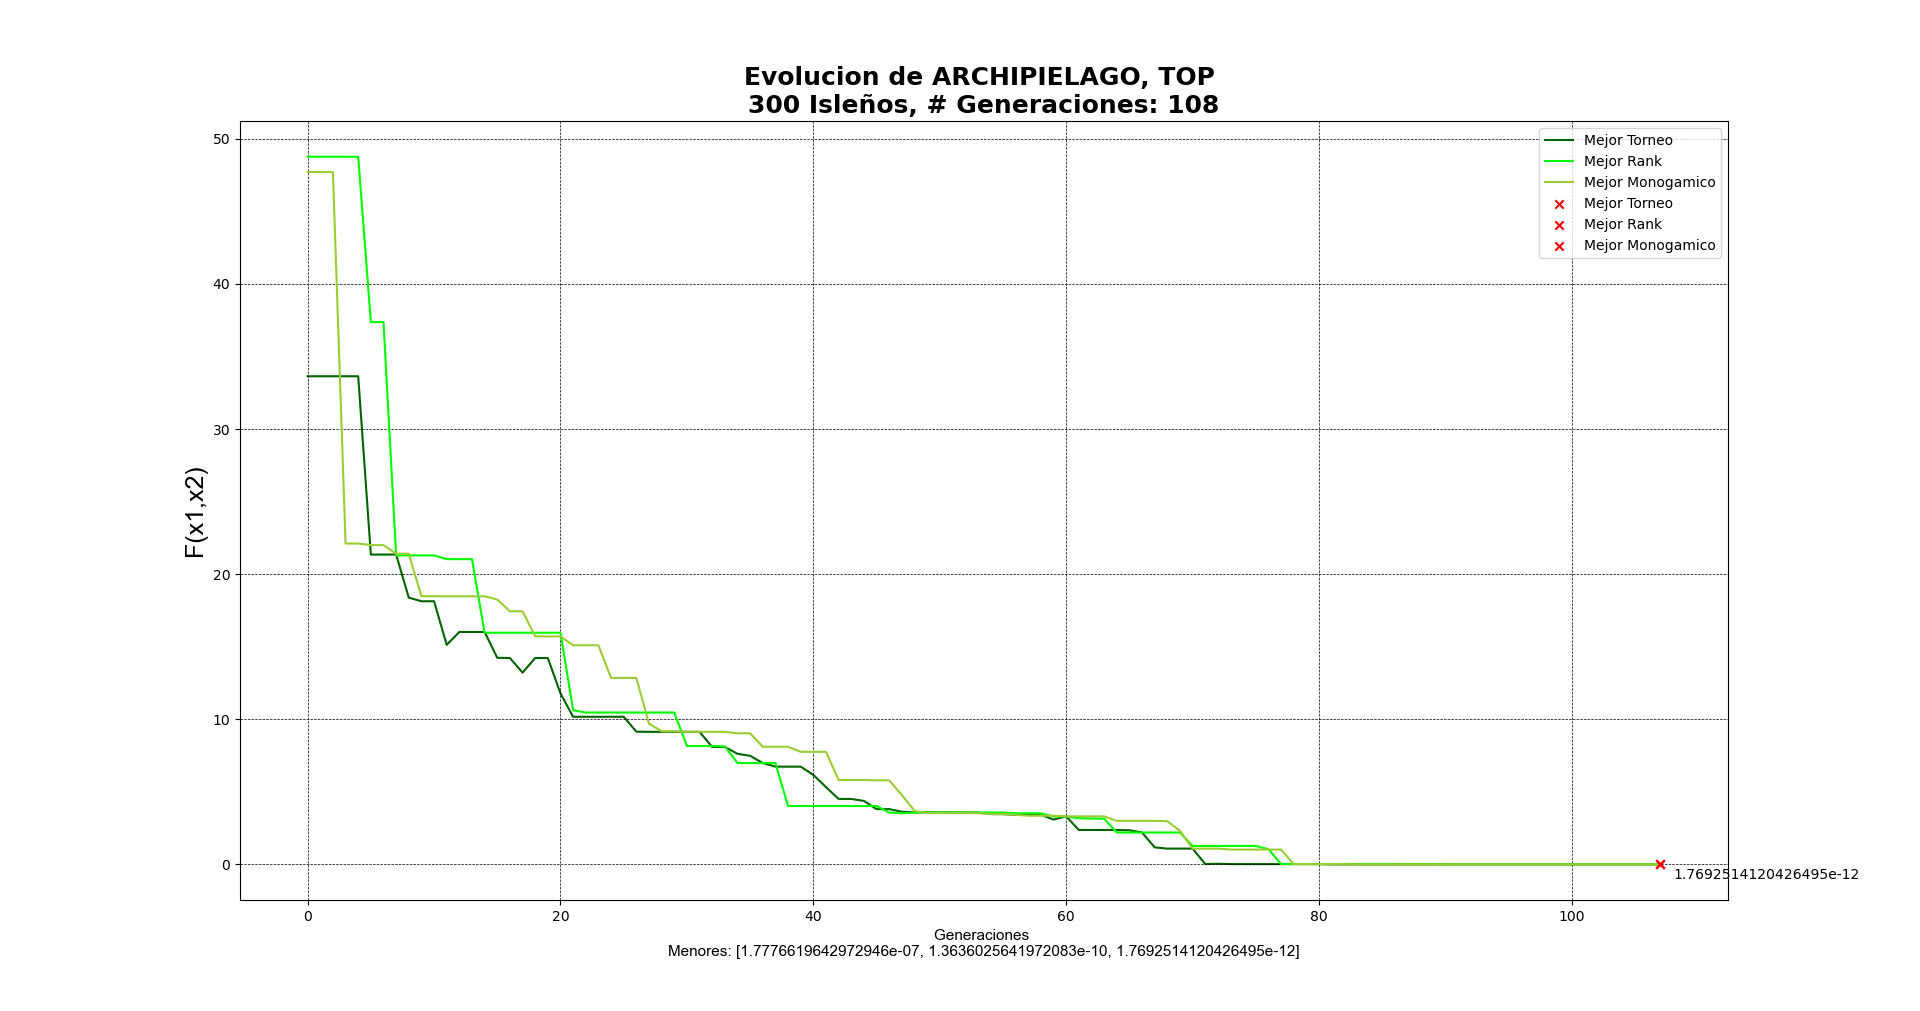
\includegraphics[width=0.85\textwidth]{C:/Users/anton/Documents/MCIA/UAQ _MCIA/Sem2_Computo_Evolutivo/Prac05_Multi-IslandAGs/Images/Figure_24.png}
            \label{Señal 2}}
        \caption{Evolucion del mejor de las islas}
        \label{Patron de señales para reconocimiento de señal Gaussiana}
      \end{center}
    \end{figure}

Parametros establecidos para prueba 3 son:
\\
\textbf{Isla 1:} Numero de Isleños: 500\\
Seleccion: Torneo\\ 
Tipo de cruza: cruza 2 puntos\\
Tipo de mutacion: Inversion de Alelos\\
\textbf{Isla 2:} Numero de Isleños: 500\\
Seleccion: Torneo\\ 
Tipo de cruza: cruza N puntos\\
Tipo de mutacion: Scramble\\
\textbf{Isla 3:} Numero de Isleños: 500\\
Seleccion: Torneo\\ 
Tipo de cruza: cruza 2 puntos\\
Tipo de mutacion: Scramble

\begin{figure}[H]
      \begin{center}
        \subfigure[Seleccion Torneo]{
            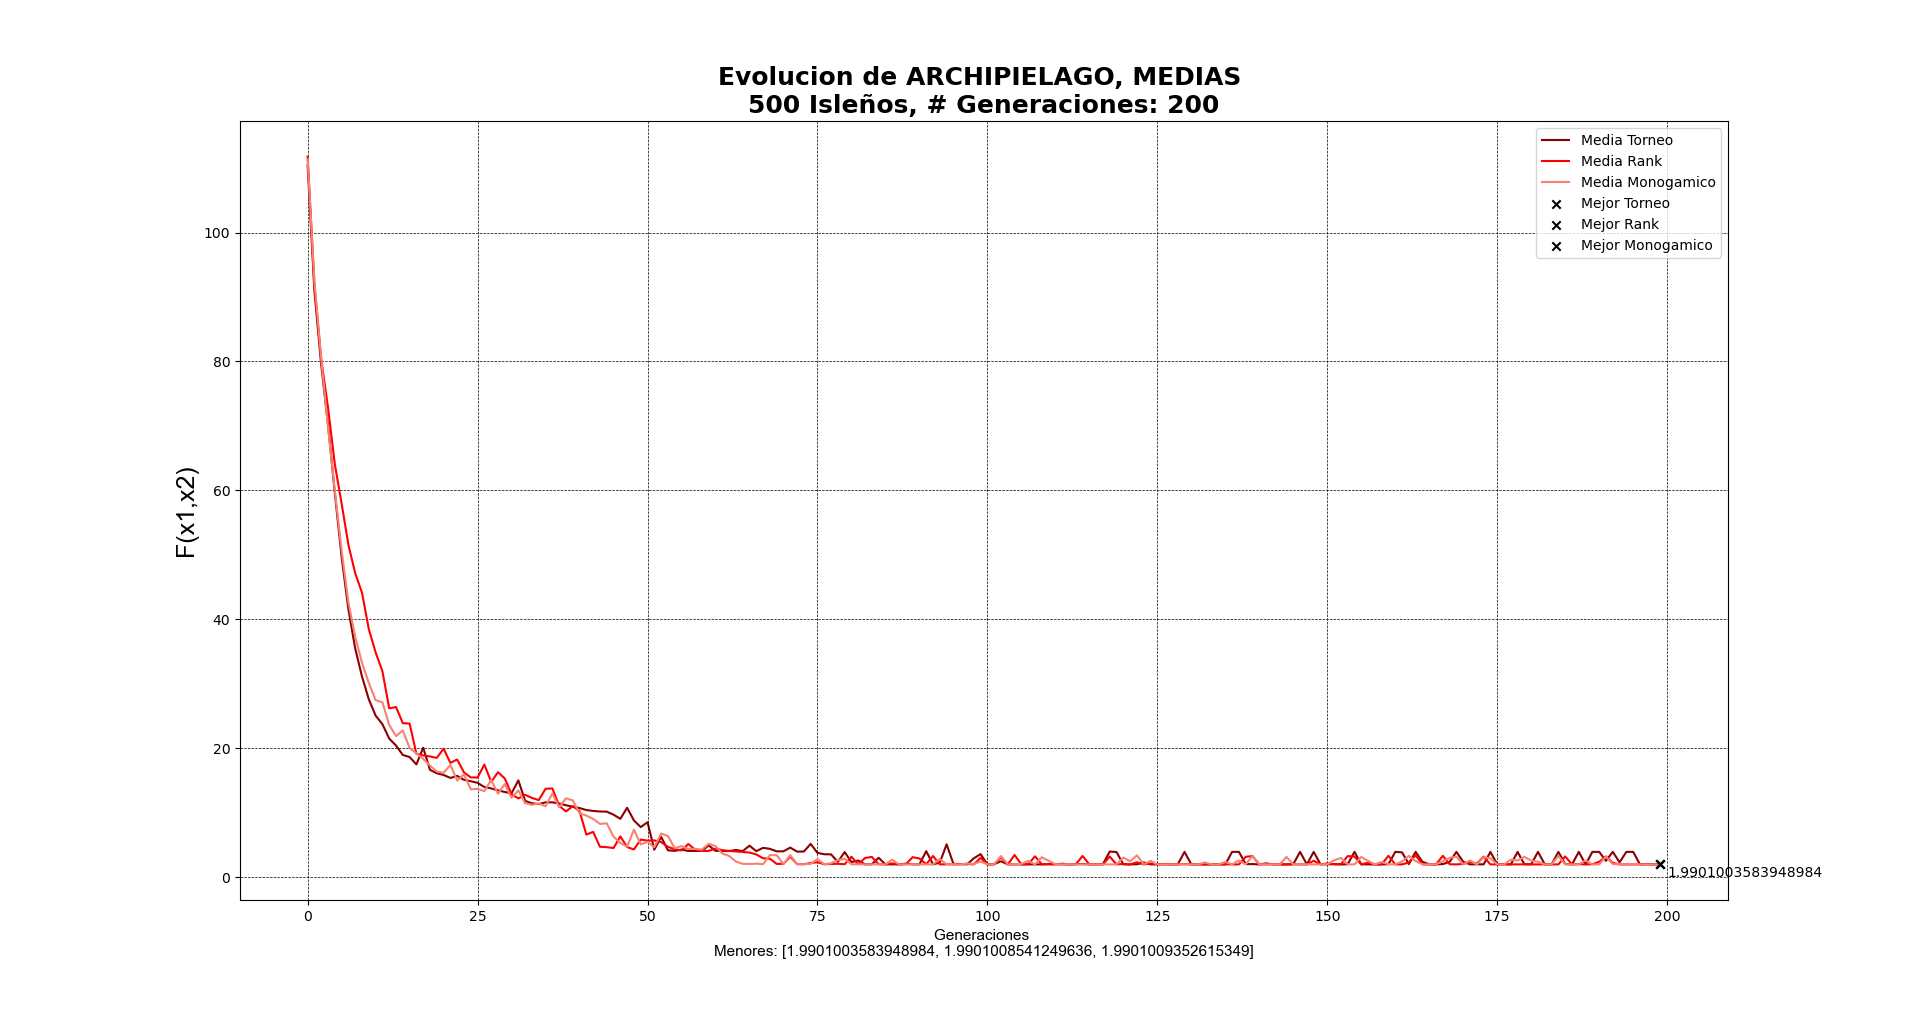
\includegraphics[width=0.85\textwidth]{C:/Users/anton/Documents/MCIA/UAQ _MCIA/Sem2_Computo_Evolutivo/Prac05_Multi-IslandAGs/Images/Figure_27.png}
            \label{Señal 1}}
        \subfigure[Evolucion de las medias de las islas]{
            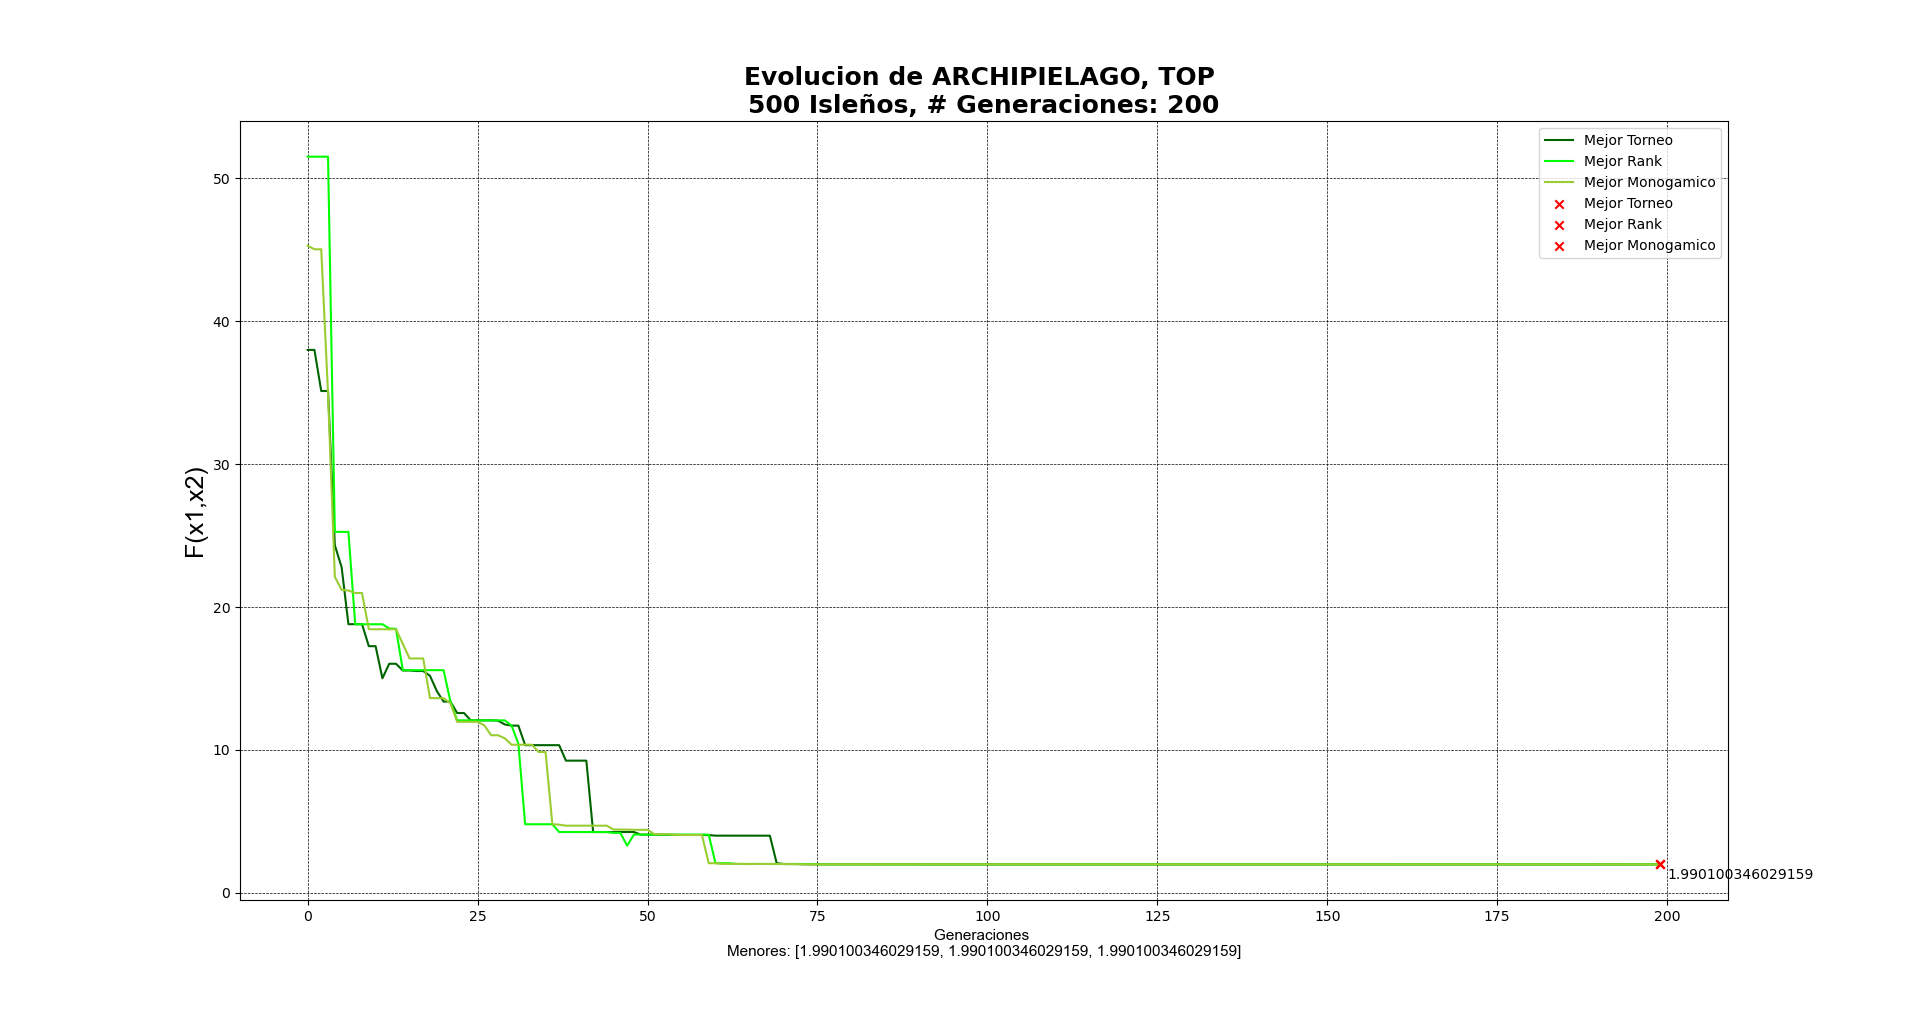
\includegraphics[width=0.85\textwidth]{C:/Users/anton/Documents/MCIA/UAQ _MCIA/Sem2_Computo_Evolutivo/Prac05_Multi-IslandAGs/Images/Figure_28.png}
            \label{Señal 2}}
        \caption{Evolucion del mejor de las islas}
        \label{Patron de señales para reconocimiento de señal Gaussiana}
      \end{center}
    \end{figure}

Parametros establecidos para prueba 4 son:
\\
\textbf{Isla 1:} Numero de Isleños: 100\\
Seleccion: Torneo\\ 
Tipo de cruza: cruza 2 puntos\\
Tipo de mutacion: Scramble\\
\textbf{Isla 2:} Numero de Isleños: 100\\
Seleccion: Torneo\\ 
Tipo de cruza: cruza 2 puntos\\
Tipo de mutacion: Scramble\\
\textbf{Isla 3:} Numero de Isleños: 100\\
Seleccion: Torneo\\ 
Tipo de cruza: cruza 2 puntos\\
Tipo de mutacion: Scramble

\begin{figure}[H]
      \begin{center}
        \subfigure[Seleccion Torneo]{
            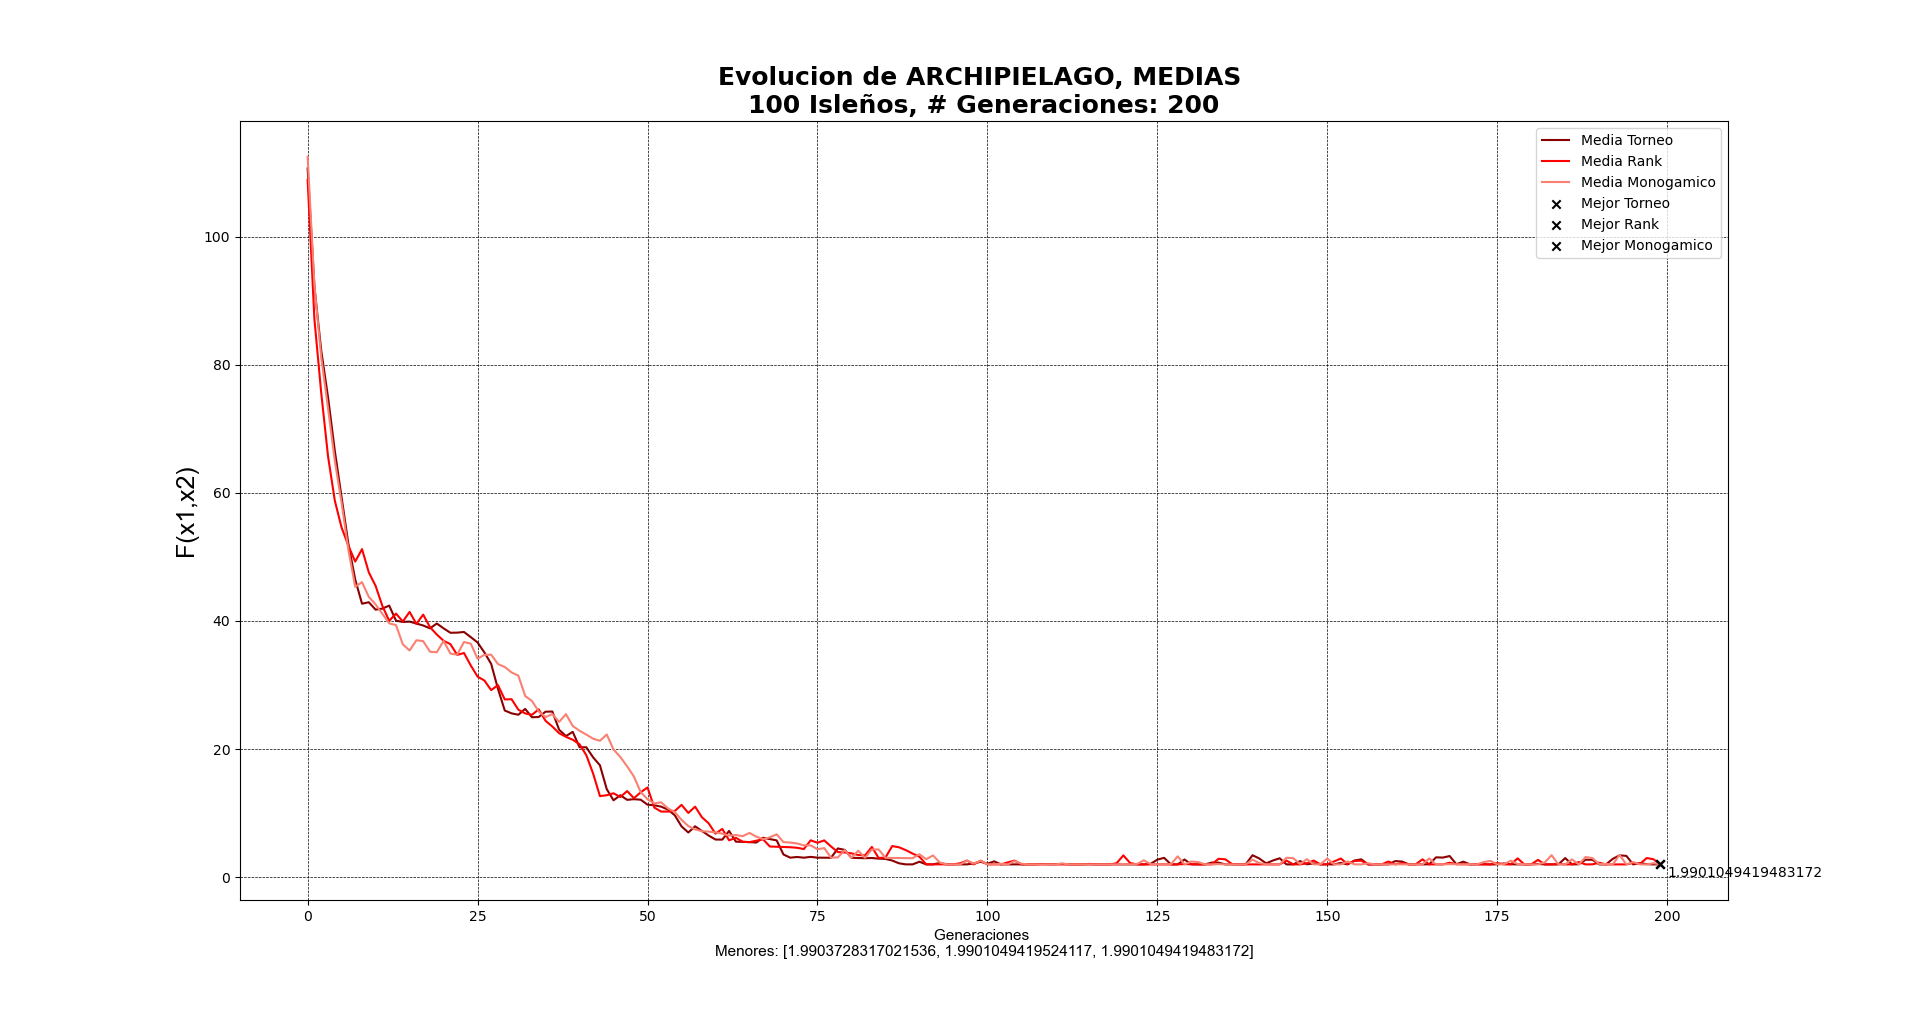
\includegraphics[width=0.85\textwidth]{C:/Users/anton/Documents/MCIA/UAQ _MCIA/Sem2_Computo_Evolutivo/Prac05_Multi-IslandAGs/Images/Figure_31.png}
            \label{Señal 1}}
        \subfigure[Evolucion de las medias de las islas]{
            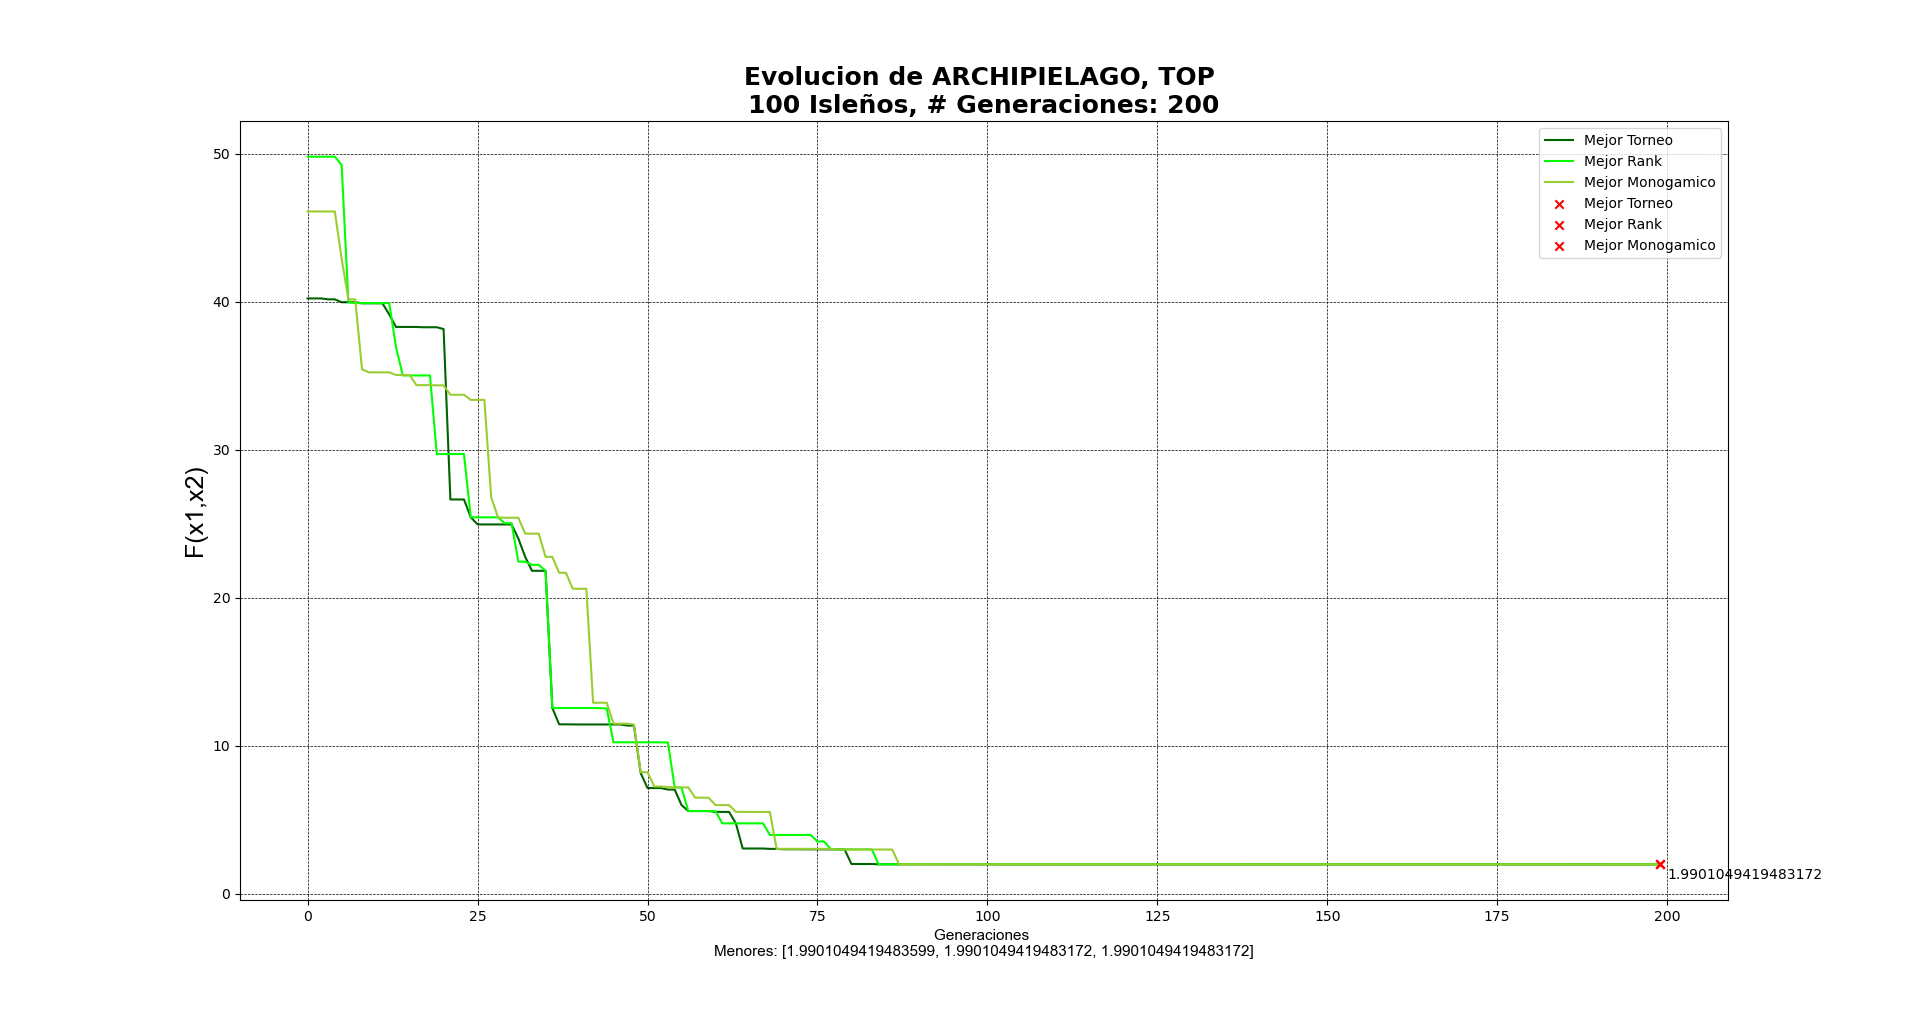
\includegraphics[width=0.85\textwidth]{C:/Users/anton/Documents/MCIA/UAQ _MCIA/Sem2_Computo_Evolutivo/Prac05_Multi-IslandAGs/Images/Figure_32.png}
            \label{Señal 2}}
        \caption{Evolucion del mejor de las islas}
        \label{Patron de señales para reconocimiento de señal Gaussiana}
      \end{center}
    \end{figure}

\section{Conclusiones}
A partir del las graficas realizadas sin migracion entre islas se observa que dificilmente alcanzan o se acercan al minimo global de $F(X)= 0$. Se observa que la mutacion de inversion de Alelos es el que peor desempeño tienen al igual que la seleccion Random Monogamica, sin embargo, la Seleccion Random Monogamico se desempeña bien cuando se selecciona con la mutacion Scramble. 
\\\\
Para todas las pruebas sin interaccion entre islas se observa que el incremento de isleños no muestra mejoria alguna para alcanzar el optimo, esto se demuestra con la grafica que tiene seleccionados los mejores tipos de cruza y mutacion y se observa que tiene el mismo desempeño que cualquier otra seleccion de parametros. Esto indica que los isleños dentro de cada isla convergen dentro de minimos locales y ya no pueden salir.
\\\\
Por otro lado, cuando se realizan las pruebas bajo las mismas condiciones pero con migracion entre islas se observa que incluso en una prueba se alcanza el minimo de tolerancia lo que claramente indica que alcanzo el minimo global que es lo mas cera de 0 posible. Ademas se observa una evolucion mucho mas rapida, suave y casi igual entre cada isla, por lo que compartir informacion entre ellas es un factor a tomar, debido a que alguna isla por mas peor que este su promedio puede contener alguna informacion que se acerque por otro lado al minimo global.
\\\\
Ademas se verifica que las 3 islas alcanzan un mínimo global similar, que si bien no es el mas bajo no distan mucho uno de la otra consiguiendo resultados en generaciones menos prolongadas.

\begin{thebibliography}{0}
	\bibitem{} Anna Demidova, Global Optimization Software and Evolutionary Algorithms, Lomonosov Moscow State University, 119991, Moscow, Russia
	\bibitem{} M. Yousaf., (2017), Genetic Algorithm for Traveling Salesman Problem with Modified Cycle Crossover Operator., Computational Intelligence and Neuroscience., Research Article., 7430125., 7 Pages.
\end  {thebibliography}

\section{Anexos}
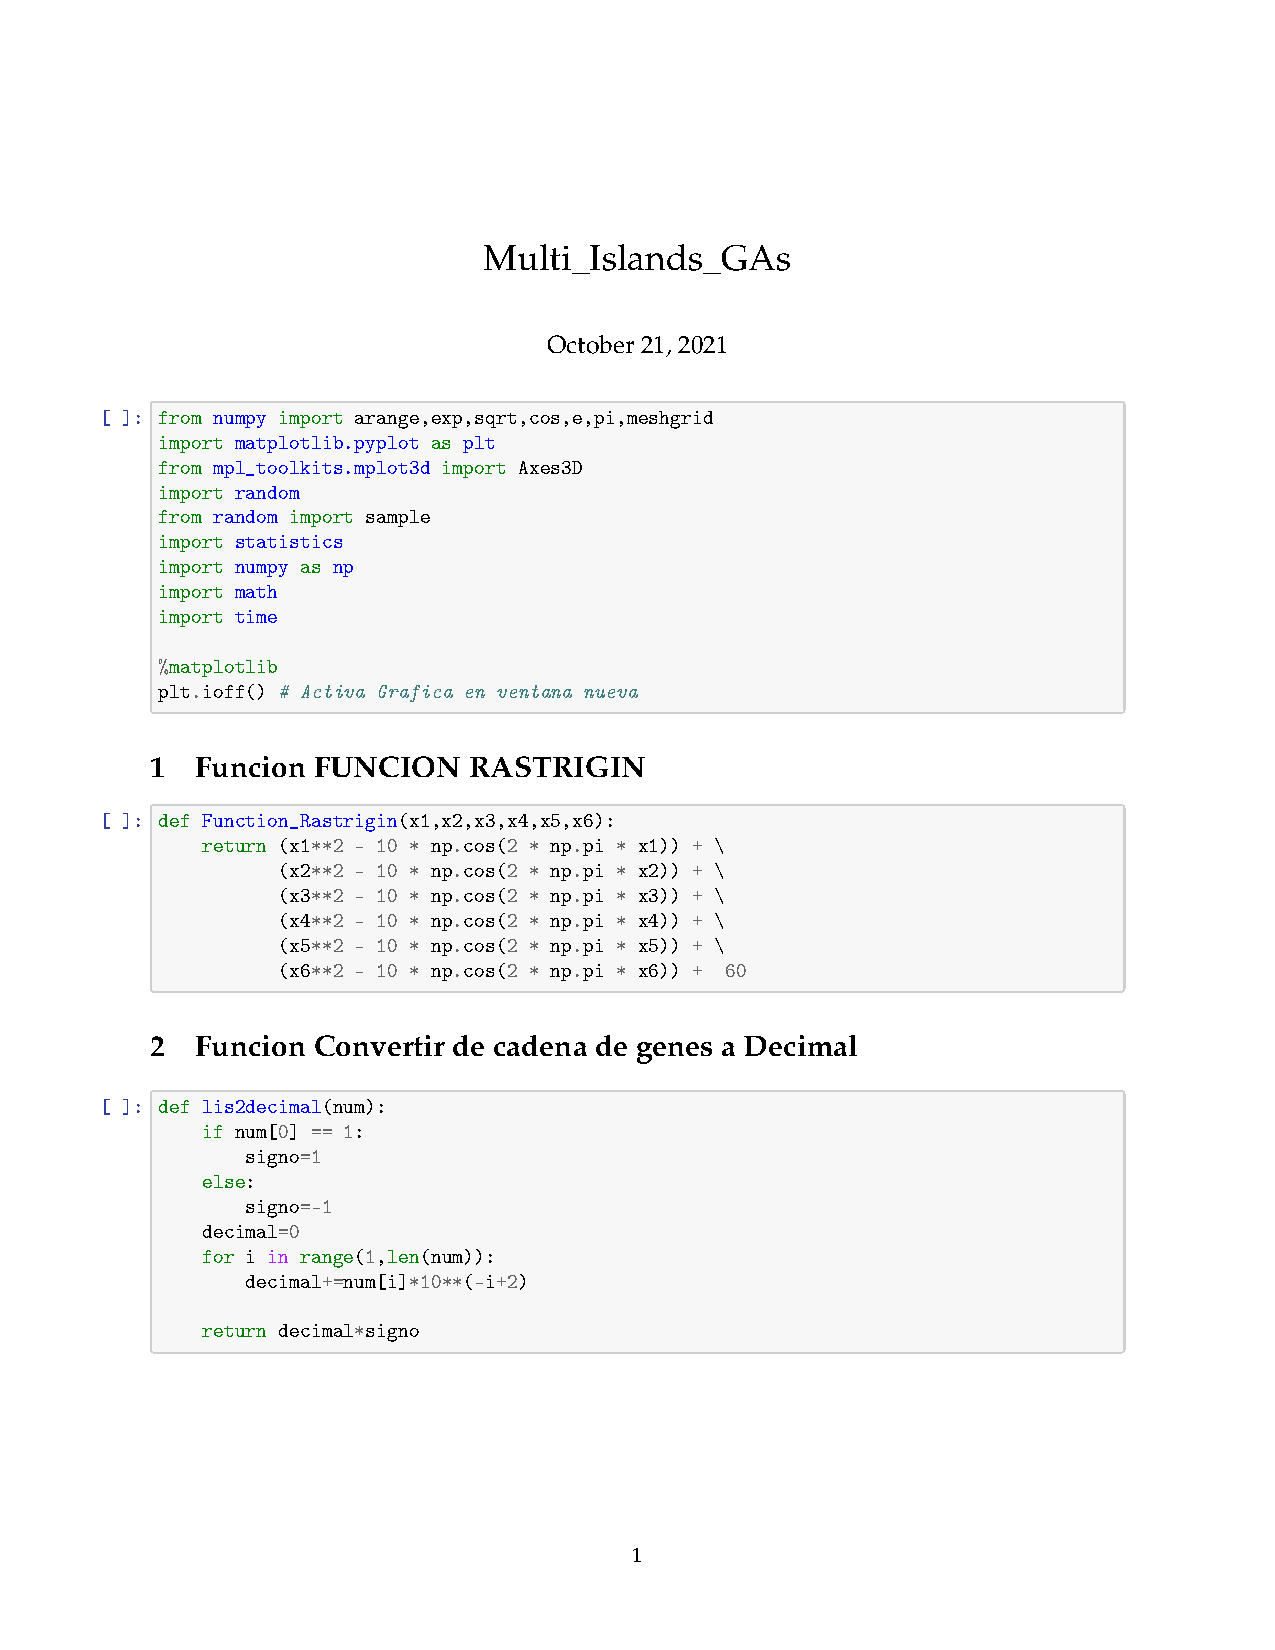
\includepdf[pages=-]{Multi_Islands_GAs.pdf}
\end{document}